\documentclass[11pt,a4paper,openleft]{book}
\usepackage[utf8]{inputenc}
\usepackage[sort]{cite}
\usepackage[english]{babel}
% \usepackage{amsmath}
\usepackage[onehalfspacing]{setspace}
\usepackage{mathtools}
\usepackage{amsfonts}
\usepackage{amssymb}
\usepackage{upgreek}
\usepackage{graphicx}
%\usepackage{floatrow}
\usepackage{lmodern}
\usepackage[dvipsnames]{xcolor}
\usepackage{transparent}
\usepackage[top=2cm, bottom=2cm, inner=2cm, outer=3cm]{geometry}
\usepackage{bm}
\usepackage{multirow}
\usepackage[font=small,labelfont=bf]{caption}
\usepackage{subcaption}
\usepackage{tikz}
\tikzset{>=latex}
\tikzstyle{vertex}=[circle, draw, thick, inner sep=0pt, minimum size=20pt]
\newcommand{\vertex}{\node[vertex]}
\usepackage{hyperref}
\usepackage{fancyhdr}
\pagestyle{fancy}
\fancyhf{}
\fancyhead[LO]{\nouppercase\leftmark}
\fancyhead[RE]{\rightmark}
\fancyfoot[LO]{\thepage}
\fancyfoot[RE]{\thepage}
\captionsetup{figurename=Figure,position=above}
\usepackage[toc,page]{appendix}
\usepackage{array}
\newcolumntype{L}[1]{>{\raggedright\let\newline\\\arraybackslash\hspace{0pt}}m{#1}}
\newcolumntype{C}[1]{>{\centering\let\newline\\\arraybackslash\hspace{0pt}}m{#1}}
\newcolumntype{R}[1]{>{\raggedleft\let\newline\\\arraybackslash\hspace{0pt}}m{#1}}
\makeatletter
\newcommand{\thickhline}{%
	\noalign {\ifnum 0=`}\fi \hrule height 1pt
	\futurelet \reserved@a \@xhline
}
\newcolumntype{"}{@{\hskip\tabcolsep\vrule width 1pt\hskip\tabcolsep}}
\makeatother

\setlength{\parindent}{0.1cm} %no indent for the paragraphs

\author{Fabian Farina}
\title{Attractors and their Basins of Attraction in Random Boolean Networks}

\begin{document}
	%titlepage
	\thispagestyle{empty}
	\newgeometry{top=2cm, bottom=2cm, inner=2cm, outer=2cm}
	\begin{center}
		\begin{minipage}{0.85\linewidth}
			\centering
			%University logo
			%\includegraphics[width=0.3\linewidth]{logo.pdf}
			\vspace*{3.5cm}
            {{\Large Goethe University Frankfurt\\
            		\vspace*{0.2cm}
            		\large Faculty of Physics\\
            		Institute for Theoretical Physics\par}}
			%Thesis title
			\vspace*{2.5cm}
			{\large Master Thesis\par}
			\vspace*{1.5cm}
			{{\Large Attractors and their Basins of Attraction in Random Boolean Networks\par}}
			\vspace*{3cm}
			{Author:\\
				Fabian Farina\par}
			\vspace{1cm}
			%Author's name
		    \begin{minipage}{0.645\linewidth}
		    	{Supervisor:\\
		    		Prof. Dr. Claudius Gros\par}
		    \end{minipage}
	    \begin{minipage}{0.345\linewidth}
	    	{\flushright Second Assessor:\\
	    		Prof. Dr. Jochen Trieschblocksatz\par}
	    \end{minipage}
        \begin{minipage}{\linewidth}
        	{\centering\vspace{3.5cm}
        		%Date
        		{\Large January 2021}\par}
        \end{minipage}
		\end{minipage}
	\end{center}
	\clearpage
	\restoregeometry
\newpage
\thispagestyle{empty}
\clearpage
\tableofcontents
\thispagestyle{empty}
\clearpage
\thispagestyle{empty}
\clearpage

\setcounter{page}{1}

\chapter{Introduction}\thispagestyle{fancy}
\paragraph*{}
If you have ever encountered a scientific publication that touches on a biological topic from the viewpoint of complex systems, you will most likely have come across a line like this: "Life lies on the edge of chaos."

\paragraph*{}
This sentence might seem to be a philosophical statement to someone outside of this field and even sound a little bit esoteric. When in reality, it is nothing than a well-grounded scientific hypothesis. It relies on the observation that many complex systems have two different poles of behavior for certain values of their underlying parameters. On the one side of the spectrum, we have almost perfect predictability and everything seems to be kind of boring because not much is happening at all. On the opposite of this, dynamical systems can behave almost randomly and there seems to be not much long-term predictability left.


\paragraph*{}
Both of those dynamic characteristics are not very suitable for life. It is a constantly changing process but not one where all previous information is irrelevant and can be lost. But there exists something in between, a border that separates the frozen and the chaotic phase. Systems that lie exactly on this border are called critical. They do not behave simply as a combination of the other two phases but rather exhibit some characteristics uniquely belonging to them. Their dynamics are often fairly complex, but not to the degree to which we would also view them completely random. Therefore, critical systems seem to be a reasonable place for finding models that describe biological processes.

\paragraph*{}
Random Boolean networks are a prototypical example of complex time-discrete dynamical systems. Moreover, they have been proposed as a first-order approximation of gene regulatory networks by S. Kauffman \cite{kauffman1969metabolic} in 1969. To be a little more specific, he did not actually invent them but rather defined a specific type of them, which he viewed as capable of modeling their biological counterparts.\footnote{The idea of studying boolean networks originated in 1966 and was first published by C. Walker and W. Ashby \cite{walker1966temporal}. In the literature, they are often not even mentioned and S. Kauffman is falsely credited to be their inventor. He was instead the first one studying them thoroughly and only through his work they gained the popularity they had in the second half of the 20th century.} During morphogenesis, genes can be viewed as being either expressed or not. How they change over time depends on the expression levels of a few other ones. Those dependencies define a network structure and the influence the genes have on each other can be modeled as Boolean functions.

\paragraph*{}
This description is a heavy simplification of the real biological process. Still, it is already sufficient to demonstrate stability, similar to the behavior observed in real cells, which S. Kauffman already noticed in his previously mentioned work. This given perspective on Boolean networks is only a little motivation and provides an argument for the relevance of studying such systems in the first place. But as this thesis belongs in the field of physics, this is as far as we will go with the biological background. 

\paragraph*{}

We will be focusing on the model itself and study its properties. It is not limited to the cell processes and could easily describe some phenomena of, for example, social interactions and other interesting topics. We started our studies with the main focus on critical networks but realized that it is more useful to consider systems in all phases and draw direct comparisons. Our main goal was to observe different statistical properties of attractors and their stability under the influence of noise. To understand random Boolean networks, we do not assume any previous familiarity with the topic and therefore introduce all necessary background knowledge.

\paragraph*{}
The first section is a general take on discrete dynamical systems. We define them and explain what attractors are and the stability of them. Thereafter we provide a brief introduction to probability theory and introduce random variables to define the expected value and its standard deviation, which we use throughout our whole work. The third section is about graphs and defines nodes, edges and the degree of a node. In those first three sections, we limited ourselves only to the relevant things for random Boolean networks. But even though we did not need it for our studies, we also had to include some definitions, like the adjacency matrix of a graph, since one will definitely be confronted with it in the literature.

\paragraph*{}
The fourth section is about binary logic and is comparably longer than what you would find in other works on random Boolean networks. But we felt that this is an unjust under\-representation of this field since it is actually useful for a better understanding and therefore decided to present it like this anyway. Here we introduce boolean variables, explain how to work with them in general and in the end, define boolean functions. This approach came in quite handy when developing and testing the algorithms that we build for our simulations.


\paragraph*{}
After this preparation, the last two sections of this chapter are about the random Boolean network model. We start by collecting the relevant things from the previous sections to define it. Then we go through an example network and thereby learn about the dynamics of it. Here we come across the concepts of attractors, their basins of attraction and garden-of-Eden states. 

\paragraph*{}
Since we are mainly concerned with ensembles of networks rather than individual realizations, the last section goes through the details of this and gives an outlook on what to expect. We specify the different ways to let the machine sample through random network realizations. Namely how to decide on the graph structure and choosing the boolean functions. The hamming distance is introduced as a useful tool for observing how different two states are compared to each other. Also, we define ergodic sets, which we will come across in our main work.

\paragraph*{}
After the theoretical background has been built up, we come to our main work in Chapter 3. We use the model introduced by S. Kauffman. Therefore we start by looking at the networks' topological structure and compare the node degree to the theoretically predicted Poisson approximation. The section afterward is on the dynamical differences for networks in the different phases. We reproduce the development of the Hamming distance for two slightly different states over time, which is a well-known aspect of random Boolean networks throughout the literature.

\paragraph*{}
To gain further insights into the dynamics of our model, we also introduce the annealed approximation. It can be used to predict the growth of the Hamming distance of two consecutive time steps for networks in the chaotic phase. We also compare this theoretical result to what can be observed for the real networks and find that it is pretty accurate.

\paragraph*{}
Right thereafter, we will come to the essential part of our research. We study the attractors and, more specifically, the averages of the basins' sizes and especially look at how the length or the number of attractors in a single realization influences it in all different phases and analyze the garden-of-Eden states. 

\paragraph*{}
We will find that the chaotic phase behaves in a way that is most similar describable to a random walk with no repetition over a finite number of elements. On the other hand, the frozen systems are boring because the dynamic dies out rather quickly and there is not too much happening at all with them. The exact values we find are still interesting and can be compared to what we figured out for the critical systems.

\paragraph*{}
The sizes of the basins of attraction for critical networks can best be explained with independent subsystems and their subattractors. Those influences the number of attractors one can observe in a single realization on average, which determines the size of the basin of attraction. As a general rule, it can be stated that the more attractors a run has, the smaller its basin gets.

\paragraph*{}
In the last part, we also wanted to know more about the attractor's stability and analyze the effect that single node flips have on the dynamic. More specifically, we divide the nodes into the frozen and not-frozen ones, which means if they change between the cycle states. We could observe that there is almost no difference between the node groups for critical networks, though the frozen ones are a little bit more stable. In the frozen phase, the frozen nodes are much more stable and in the chaotic phase, the active ones are more so, even though they are overall much less stable than the other networks.

\paragraph*{}
We tried to maintain balance in providing enough background information that even someone unfamiliar with the topic will understand it with minimal prerequisites and, on the other hand, pointing out where our personal contributions to the field lie. Therefore, the first half focuses on all kinds of definitions and gives some examples to understand the dynamic of random Boolean networks. The second half contains the results of all our simulations, which are both: reproduction of known behavior and our very own results. The latter have to our best knowledge not been done somewhere before and could not be found throughout the literature. In the end, we will shortly recapitulate all this and give some ideas for how to go further with the research starting from our work.

\newpage
\thispagestyle{empty}

\chapter{Theoretical Background}\thispagestyle{fancy}
\section{Discrete Dynamical Systems}

\paragraph*{}
Dynamical system theory is a vast field, with various applications in natural and social sciences. It uses all kinds of mathematical concepts from different areas, but to maintain clarity throughout this work, we will only focus on the necessary definitions in this section. In the most general sense the theory is about modeling systems, especially how a certain set of its variables $ \boldsymbol{x} = \{x_1,\dots,x_N\} $ evolves over time. A more precise definition of a set will be given in the next section, but for now it is simply the collection of those variables. 

\paragraph*{}
Classically, the theory of dynamical systems deals only with a hand full of variables. However, in nature, we often have many separate parts that interact with each other. Because of this, the theory of complex systems evolved. With it, theorists try to deduce seemingly complicated collective behavior as an emergent property of the rules the part taking components have to obey. The random Boolean networks (RBNs) on which this thesis is mainly about, can be seen as a prototypical complex system. Many properties can be derived analytically for it and it shows many phenomena other complex systems also have. That is why scientists studied RBNs extensively and many reviews on them have been written by now, for example, M. Aldana et al. \cite{aldana2003boolean} or B. Drossel \cite{drossel2008random}. We will return to them later on when we have provided the necessary knowledge to understand such networks properly.

\paragraph*{Dynamical Systems}
One major separation between different classes of models of dynamical systems is the way how time gets defined. Here it will only be discrete and can be associated with the natural numbers: $ t \in \mathbb{N} $. Let the phase space $ \mathcal{X} $ be the set of all possible values the variables $ \boldsymbol{x} $ can have and define the map $ \phi :  \mathcal{U}\subset\mathcal{X} \longrightarrow \mathcal{X} $ with $ \boldsymbol{x} \mapsto \phi (\boldsymbol{x}) $. It will be chosen in a way, that the following equation then defines the dynamical system and its behavior for all times:
\begin{equation}
\boldsymbol{x}_{t+1} = \phi(\boldsymbol{x}_t).
\end{equation} 
The indices denote the point in time of the variables. This notation is commonly used for systems with discrete-time evolution and will be used equivalently to the continuous one. Thus we will use $ x(t) $ and $ x_t$ interchangeably.

\paragraph*{Fixpoints}
There are many ways the parameters could be evolving. They could, for example, only grow, decrease or do both and maybe oscillate. One interesting thing is fixpoints and limit cycles. If there exists a point $ \boldsymbol{x}^*\in \mathcal{X} $, it will be called a fixpoint, if it fulfills the following equation:
\begin{equation}\label{eq:fixpoint}
\boldsymbol{x}^*=\phi(\boldsymbol{x}^*).
\end{equation}

\paragraph*{}
Once the system reaches this point, it stays for all following time steps at it. If the map $ \phi $ has a first derivative with respect to time, the stability of this fixpoint could be further analyzed analytically. But since this is not always the case, as it happens to be in our model as well, we first want to define stability in a dynamical manner. If there exists at least one $ \boldsymbol{x}_0\in \mathcal{X} $, such that 
\begin{equation}\label{eq:stable_fixpoint}
\lim\limits_{t\rightarrow \infty} \phi^t (\boldsymbol{x}_0) = \boldsymbol{x}^*\text{ and } \boldsymbol{x}_0 \neq \boldsymbol{x}^*,
\end{equation}
the fixpoint will be called stable. This equation is analogous to the notion, that the phase space contracts around $ \boldsymbol{x}^* $ in a continuous time system. Note that the superscript over the map is not a power and means instead $ t $ times its composition:
\begin{equation}
\phi^t (\boldsymbol{x}) := \underbrace{(\phi \circ\dots\circ\phi)}_{t\text{ times}}(\boldsymbol{x}).
\end{equation}

\paragraph*{}
We will continue with the analysis of stability, but first, we have to introduce cycles since their concept is closely related to fixpoints.

\paragraph*{Cycles}
Another possible behavior of the system would be for it coming back to a previous state $ \boldsymbol{x}_1\in \mathcal{X} $ after $ L $ time steps:
\begin{equation}
\boldsymbol{x}_1 = \phi^L(\boldsymbol{x}_1).
\end{equation}
Of course, this implies that $ L $ is the shortest number of steps, where this equation holds. From this chain it is possible to construct the series $ \left(\boldsymbol{x}_1,\phi(\boldsymbol{x}_1),\dots,\phi^{L-1}(\boldsymbol{x}_1) \right) \in \mathcal{X}^L $, which will be called a cycle $ C_L $ of length 
$ L $. It is not important from which state the cycle starts. What matters is its order and size. If equation (\ref{eq:stable_fixpoint}) holds for at least one element of the cycle, then it is also called stable. A cycle with $ L=1 $ is just a fixpoint. The more general term is attractor, whenever we talk about either a stable fixpoint or a stable cycle.

\paragraph*{Stability}
We now apply the phase space with a metric $d : \mathcal{X}\times\mathcal{X} \longrightarrow [0,\infty) $, with which we can measure distances between two elements of it. From it we define the norm as the distance of some element $x$ to the zero element: $\|x\|:=d(0,x)$. We further assume that the phase space is linear and derivations can be properly defined on it. More information on those topics can be found virtually in every introductory course on vector spaces or related topics in the literature, so this is as much as we need to know for now. 

\paragraph*{}
With this, we can further analyze the stability of a found fixpoint $x^*$ for a given dynamical map $\phi$ in a single dimension. Let us say that at time $t$, we are the smallest possible distance away from $x^*$:
\begin{equation}
\Delta x_t := x_t-x^*.
\end{equation}
We use this for a tailor expansion of the evolution map at the fixpoint:
\begin{equation}
\begin{split}
x_{t+1}& = \phi(x_t) = \phi(x^*+\Delta x_t)\\
& = \phi(x^*) + \phi'(x^*)\Delta x_t + O(\Delta x_t^2)\\
& = x^* + \phi'(x^*)\Delta x_t + O(\Delta x_t^2),
\end{split}
\end{equation}

\paragraph*{}
To drop the terms of higher-order $\Delta x_t$ has to be smaller than one, but even if it is not, we can substitute the variables and reformulate the problem in a way where this is given. By doing so, we end up with a relation from which we can deduce the stability of the fixpoint: 
\begin{equation}
\frac{\Delta x_{t+1}}{\Delta x_{t}} = \phi'(x^*).
\end{equation}

\paragraph*{}
If this is smaller than one, our distance to the fixpoint will decrease over time until we arrive at it. Thus we call it stable. If for every time-step, the distance keeps growing, we would call it unstable. To summarize this up, we have:
\begin{equation}\label{eq:fixpoint_stability}
\begin{split}
\|\phi'(x^*)\| < 1 & \Longleftrightarrow x^* \text{ is stable,} \\
\|\phi'(x^*)\| > 1 & \Longleftrightarrow x^* \text{ is unstable.}
\end{split}
\end{equation}

If we get exactly the value of one, we would have to gather additional information. We could maybe try to analyze the fixpoint's stability in the way we introduced its concept earlier and use equation (\ref{eq:stable_fixpoint}). This topic is closely related to the so-called Lyapunov exponents. We could introduce the idea of eigenvalues and how to use them to analyze the system even further. But since we will gain little to no more insights on random boolean networks, which are the main topic of this thesis, we will simply leave it like this and continue with other more relevant definitions.

\section{Probability Theory}
\paragraph*{}
We will later look at large ensembles and assign probabilities to certain properties of them. To define what this means, we will provide a short introduction in this section. There are many modern approaches to probability theory and for a more comprehensive introduction, we refer to the books of  A. Klenke \cite{klenke2013probability} and B. R. Bhat \cite{bhat2007modern}. For our purposes, it is enough to reduce ourselves to naive set theory as our basis.

\paragraph*{Sets}
Any unordered collection of elements will be called a set $\mathcal{S}$. If $x$ is an element in $\mathcal{S}$, we write $x\in \mathcal{S}$. For example and further definition, let $a$ and $b$ form the set $\mathcal{S}:=\{a,b\}$. As such it has to be idempotent, meaning that $\{a,a,b\} = \{a,b\}$ and symmetric, such that $\{a,b\} = \{b,a\}$. If all the elements of set $\mathcal{A}$ are also elements of the set $\mathcal{B}$, we call $\mathcal{A}$ a subset of $\mathcal{B}$ or $\mathcal{A}\subseteq\mathcal{B}$. It is obvious, that any set $\mathcal{S}$  has to be a subset of itself $\mathcal{S}\subseteq\mathcal{S}$. If we have $\mathcal{A}\subseteq\mathcal{B}$ and $\mathcal{A}\neq\mathcal{B}$, then $\mathcal{A}$ is a proper subset of $\mathcal{B}$. Since we can not always list all the elements of a set in order to define it, a common way of doing this would be to write 
\begin{equation}
\mathcal{S}:=\{x|x\text{ has property }y\}
\end{equation}
for a set of all elements, that are of property $y$.

\paragraph*{Operations and Special Sets}
The disjunction of two sets $\mathcal{A}$ and $\mathcal{B}$ is defined as 
\begin{equation}
\mathcal{A}\cap\mathcal{B}:=\{x|x\in \mathcal{A}\text{ and }x\in \mathcal{B}\}.
\end{equation}
The conjunction of them is 
\begin{equation}
\mathcal{A}\cup\mathcal{B}:=\{x|x\in \mathcal{A}\text{ or }x\in \mathcal{B}\},
\end{equation}
where "or" has to be interpreted in the sense, that $\mathcal{A}\cap\mathcal{B}\subseteq\mathcal{A}\cup\mathcal{B}$ is true. The empty set $\emptyset$ is the only set, which contains no elements. It is obvious that for all sets $\mathcal{S}$, the empty set is a subset $\emptyset\subseteq\mathcal{S}$. The power set of $\mathcal{S}$ is the set $2^\mathcal{S}$, which has as its elements all the subsets of $\mathcal{S}$. Another common way of writing this would be $2^\mathcal{S}:=\{x|x\subseteq \mathcal{S}\}$.

\paragraph*{Cardinality}
The cardinality of a set is the number of its distinct elements. For a set $\mathcal{S}$ it is denoted as $|\mathcal{S}|$. For the empty set it is $|\emptyset| = 0$ and for the power set of $\mathcal{S}$ it is $|2^\mathcal{S}|=2^{|\mathcal{S}|}$.

\paragraph*{Probabilities}
We are now interested in experiments and would like to assign probabilities to their possible outcomes. All of those outcomes together as a set are what we call the sample space $\Omega$. An event $\mathcal{F}$ is some subset of this sample space, that we are interested in. This lets us define the probability of an event to be happening as:
\begin{equation}
P(\mathcal{F}) := \frac{|\mathcal{F}|}{|\Omega|}.
\end{equation}

\paragraph*{}
For example, let us consider two coin flips in a row, where we want to know how likely it is, that both times they show the same side. So the sample space in this scenario would be 
\begin{equation}
\Omega = \{(heads,heads),(heads,tails),(tails,heads),(tails,tails)\}
\end{equation}
and the described event is 
\begin{equation}
\mathcal{F} = \{(heads,heads),(tails,tails)\}.
\end{equation}
Thus the probability of both coin flips showing the same side becomes $P(\mathcal{F}) = \tfrac{2}{4} = 0.5$. We define two events $ \mathcal{F}_1 $ and $ \mathcal{F}_2 $ as independent, if the following equation holds:
\begin{equation}
P(\mathcal{F}_1\cap\mathcal{F}_2) = P(\mathcal{F}_1)P(\mathcal{F}_2)
\end{equation}

\paragraph*{Random Variables}
In principal, a random variable is just a function, which takes an element or a subset from $ \Omega $ and maps it to a measurable space $ R $, which is for most purposes a subset of the real line $ \mathbb{R} $. We write it as 
\begin{equation}
X:\Omega \rightarrow R.
\end{equation}
We could reformulate the previous example as $ X(\omega) \in \{0,1,2,3\} $ with the corresponding probability of $ P(X\in \{0,3\}) := P(\mathcal{F}) $.

\paragraph*{Expected Value and Standard Diviation}
We use this to define the expected value. Let the random variable $ X $ have the $n$ real-valued outcomes $ x_1,\dots , x_n $ to which we can all apply their corresponding probabilities. The expected value than gets defined as:
\begin{equation}\label{eq:expected_value}
E[X] := \sum\limits_{i=1}^n x_i P(X=x_i) = \sum\limits_{i=1}^n x_i p_i.
\end{equation}
The right side of the equation is just a shorthand notation, which is often in use. We see that it is a linear map by definition. The expected value of an expected value is again this same expected value: $ E[E[X]] = E[X] $.

\paragraph*{}
To define the standard deviation, we start by first introducing the variance, which is the quadratic difference of the random variable around its expected value:
\begin{equation}\label{eq:variance}
\begin{split}
\text{Var}(X) &:= E[\left(X-E[X]\right)^2]\\
&= E[X^2] - E[X]^2.
\end{split}
\end{equation}
The line below the definition is a direct result derived from the properties of the expected value. We then define the standard deviation as:
\begin{equation}\label{eq:standard_deviation}
\text{Std}(X):= \sqrt{\text{Var}(X)} = \sqrt{E[X^2] - E[X]^2}.
\end{equation}
In the literature, it is often denoted as $\sigma$, but since we will use this otherwise and do not want to get too confusing with our notation, we will rather leave it like this. The standard deviation can be interpreted to measure how much we would assume the random variable to be varying around its expected value.

\paragraph*{Bernoulli Process}\label{sec:bernoulli_process}
A finite or infinite sequence of random variables with only two outcomes is called a Bernoulli process. Say we have a probability of $p \in [0,1]$ for the first event to be true. The number of times the event comes true can be considered as a new random variable $ X $. Then we can calculate the probability of it to appear $k$ times after $n$ trials in total as:
\begin{equation}\label{eq:Bernoulli}
p_k := P(X=k) = {n\choose k} p^k(1-p)^{n-k}.
\end{equation}

\paragraph*{}
It is straightforward to see why this has to be the case. Let us think of the process regarding a string with $n$ letters, which are either $a$ or $b$. The likelihood of finding the letter $a$ at a certain place would therefore be $p$. Having the first $k$ times $a$ would mean that the other $n-k$ letters have to be all $b$s. Since all letters' probabilities are independent of each other by definition, the probability of finding a string with said properties has to be the product of the individual ones. Thus finding such a string would have the probability $p^k(1-p)^{n-k}$. But this is not the only way of having exactly $k$ letters being $a$. In fact, there are ${n\choose k}$ different ways of placing the $a$s and $b$s from before in a string of length $n$. Combining this leads to equation (\ref{eq:Bernoulli}), which gets also called the binomial distribution.

\paragraph*{}
The expected value can be calculated due to the linearity property. When $ X_1,\dots , X_n $ are the random variables that describe each single outcome of the Bernoulli process, than our random variable from before is just the sum of those and as such also the expected value becomes:
\begin{equation}\label{eq:Bernoulli_expected_value}
X = \sum\limits_{i=1}^{n} X_i \implies E[X] = \sum\limits_{i=1}^{n} E[X_i] = \sum\limits_{i=1}^{n} p =np.
\end{equation}
The variance of this can be calculated with equation (\ref{eq:variance}):
\begin{equation}
\begin{split}
\text{Var}(X) &= E[X^2] - E[X]^2\\
&= \sum\limits_{k=0}^n k^2 p_k - (np)^2\\
&= \sum\limits_{k=0}^n k^2 {n \choose k} p^k(1-p)^{n-k} - n^2 p^2\\
&= np(1-p)
\end{split}
\end{equation}
Here we skipped some steps to come to the solution, but the full derivation of this can be found via a quick online-search and we would add no value to our work by copying it. The standard deviation is:
\begin{equation}
\text{Std}(X)=\sqrt{np(1-p)}.
\end{equation}

\section{Graphs and Networks}
\paragraph*{}
Networks are nowadays one of the most useful tools for structuring complex systems and making sense of them. They are of uttermost importance for modeling the human brain \cite{sanz2015mathematical}, credit relations between firms and banks \cite{gatti2006business}, understanding social interaction \cite{klemm2003nonequilibrium} and many more. Not even to mention that modern days artificial intelligence approaches are almost always a particular type of neural network. A. L. Barab\'{a}si provided an accessible introduction to network sciences \cite{barabasi2016network} on which this section is oriented.

\paragraph*{Vertices and Edges}
A network, also called a graph $G=(V,E)$ is an ordered pair containing a set of vertices (nodes) $V$ and the edges (links) 
\begin{equation}
E\subseteq\{(v_i,v_j)\ |\ (v_i,v_j)\in V^2 \wedge i,j\in\{1,\dots,N\}\}
\end{equation}
between them. We write $e_{ij}:=(v_i,v_j)$ for the edge that starts at the $j$-th and points to the $i$-th vertex. More precisely, what has been defined here is a directed graph, since the edges are ordered pairs, meaning $e_{ij}\neq e_{ji}$. For an undirected graph, the order would not matter. If $E = V^2$, we call the graph fully connected, since in this case, there are edges between all the nodes.

\paragraph*{Node Degree}
We define the in-degree of vertex $v_i$ as the number of edges pointing towards it. We will denote it by $k^{(in)}_i$. Analogously the out-degree $k^{(out)}_i$ is the number of edges starting from it. The degree $k$ of the graph as a whole is the average number of edges per vertex. Since every edge needs to have to start and end at a vertex and has to point somewhere, it is clear that the in- and out-degrees averages have to be the same: $\langle k^{(in)}\rangle=\langle k^{(out)}\rangle=k$. For the undirected case, one has not to distinguish between them at all. The in- and out-degrees of a graph can best be seen at an example like in Figure \ref{fig:graph_example}.

\begin{figure}
	\begin{subfigure}{0.5\textwidth}
		\includegraphics[width=0.9\textwidth]{Plots/graph_example}
	\end{subfigure}
	\begin{subfigure}{0.5\textwidth}
		\includegraphics[width=0.8\textwidth]{Plots/graph_example2}
	\end{subfigure}
	\caption{The graph on the left has a total of $ N = 8 $ nodes and degree average of $ k = 1.75$, thus $ 14 $ edges in total. There are two links starting from node $ 1 $ and three pointing towards it, so its degrees are $ k^{(out)}_1 = 2 $ and $ k^{(in)}_1 = 3 $. The graph on the right side is a random geometric graph, which nodes got randomly placed in the plane and if the distance of two happens to be below a certain threshold, an edge was placed between them. Those are only two illustrative examples of graphs and there are uncountable many more.}
	\label{fig:graph_example}
\end{figure}

\paragraph*{Adjacency Matrix}
An introduction to graph theory would not be complete without mentioning the adjacency matrix and its relation to the node degrees. Its elements are defined as
\begin{equation}\label{eq:adjacency_matrix}
A_{ij} =\begin{cases}
1 & \text{if $e_{ij} \in E$}\\
0 & \text{otherwise}.
\end{cases}
\end{equation}
For an undirected graph, we can calculate the in- and out-degree for the $i$-th node as
\begin{equation}
k^{(in)}_i = \sum\limits_{j = 1}^{N} A_{ij} \text{ and } k^{(out)}_i = \sum\limits_{j = 1}^{N} A_{ji}.
\end{equation}
And the number of elements in the set of all edges $ E $ simply is
\begin{equation}
|E| = \sum\limits_{i = 1}^{N} \sum\limits_{j = 1}^{N} A_{ij}.
\end{equation}
For a directed graph, this would count every edge twice. Thus one would have to take half of it to get the right cardinality of the set.


\paragraph*{}
There are numerous ways to select the edges between a given set of vertices to create a network. We could use real-life data to model it or instead randomly select two vertices at a time and connect them until one creates a network with a particular degree distribution. Those distributions are a crucial feature for differentiating between certain types of networks. Typical classes are scale-free, exponential and random graphs. The latest ones often also get called Erd\H{o}s–Rényi models, in honor of the two mathematicians who first introduced and studied them intensively \cite{erdHos1960evolution}.

\paragraph*{}
The random graphs, which are the most important ones for this work, get created by choosing the edges between all nodes with the same probability.
\section{Binary Logic}
\paragraph*{}
In ancient Greek philosophers like Socrates were already asking the ontological question what the essence of reality is and how human beings with all their flaws could possibly know if anything meaningful can understand to be a certain way and not only a product of mankind's imagination. Over two millennia have passed since and such questions are still marveling. Not arguing whether satisfying answers to those mysteries have been found so far or not, it is to acknowledge that many useful theories have been developed in the search for them. Among them are binary logic and information theory, two fields on which modern days technologies strongly depend.

\paragraph*{Boolean Variables}
Binary or often also called Boolean logic is the field that only distinguishes between two truth values: "false" and "true". To make things easier they are often represented as $ 0 $ for false and $ 1 $ is true. Without the necessity of having a semantic meaning, one can obtain reasonable rules for dealing with propositions as such. For example, assume to have a preposition or rather a Boolean variable $ A \in \{0,1\}$. A tautology $ \top $ is a statement that happens to be true no matter which actual values the underlying variables take. One of those is the statement "$ A $ or not $ A $", which is self-evidently true since there are no other choices within the binary framework of logic. The opposite of is a contradiction $ \bot $ like "$ A $ or not $ A $".

\paragraph*{Interpretation and Logical Operators}
A sentence is the combination of propositions with some logical operators. In order to give some examples, it is sufficient to first introduce the interpretation of a proposition or a sentence $ A $:
\begin{equation}
|A| := \begin{cases}
0 & \text{if $A$ is false}\\
1 & \text{if $A$ is true.}
\end{cases}
\end{equation}
This might seem to be a trivial thing to do, but with this it is possible to define logical operators in an arithmetical way. The negation is a compound sentence with one logical operator $ \neg $ which acts on a single proposition $ A $ and its truth value can be calculated to be:
\begin{equation}
|\neg A| := 1 - |A|.
\end{equation}
\paragraph*{}
With a set of only a few logical operators, it is possible to construct all other logical operators. In fact, actually a single one is enough to create every single one of them. But to understand this, it is easier to start from a different point and first define two other logical operators, which now act on two propositions $ A $ and $ B $:
\begin{align}
\text{logical "and" or conjuction:}\quad\quad |A \land B| &:= |A|\cdot|B|, \\
\text{logical "or" or disjunction:}\quad\quad |A \lor B| &:= 1-(1-|A|)\cdot (1-|B|).
\end{align}

\paragraph*{}
To construct an arbitrary logical operator of $ N \in \mathbb{N} $ propositions $ \mathcal{O}(A_1,\dots,A_N) $ one would start by considering all the combinations of truth values, which should make the operator true and connect them with the operators introduced so far. How this should be done, can be most easily demonstrated by an example. The "exclusive or" is the operator $ \oplus $, which is true if either one of its two propositions is true, but false if all of them are false or all of them are true:
\begin{equation}\label{eq:XOR}
|A_1\oplus A_2| := 
\begin{cases}
0 \quad\text{if } |A_1\land A_2| = 1 &(P1),\\
1 \quad\text{if } |\neg A_1\land A_2| = 1 &(P2),\\
1 \quad\text{if } |A_1\land \neg A_2| = 1 &(P3),\\
0 \quad\text{if } |\neg A_1\land \neg A_2| = 1 &(P4).
\end{cases}
\end{equation}

\paragraph*{}
Obviously $ |A_1\oplus A_2| $ is true, if either $ P2 $ or $ P3 $ are the case, which directly leads to another possible way of defining the operator in terms of:
\begin{equation}
|A_1\oplus A_2| = |P2\lor P3| = |(\neg A_1\land A_2)\lor (A_1 \land \neg A_2)|.
\end{equation}

\paragraph*{Adequate Sets}
With this receipt of building disjunctions of conjunctions that are true, one can easily now construct also every other logical operator. This is exactly the definition of functional (or also logical) completeness for a set of logical operators, which are in this case $ \{\neg,\land,\lor\} $. Sets that have this property are then called adequate sets. It is possible to have even smaller logical complete sets of operators. If you consider, that it is $ |A_1\lor A_2|\Leftrightarrow|\neg(\neg A_1\land\neg A_2)| $, which is basically De Morgan's law, then it follows directly, that $ \{\neg,\land\} $ is also an adequate set.

\paragraph*{}
It is even possible to have logically complete sets with only one operator. Peirce's arrow $ \downarrow $ for example is only true, if both of its propositions are false. With this definition it is not too hard to check for the two propositions $ A_1 $ and $ A_2 $, that:
\begin{align}
|\neg A_1| \quad &\Leftrightarrow\quad |A_1 \downarrow A_1|,\\
|A_1\land A_2| \quad &\Leftrightarrow\quad |(A_1\downarrow A_1)\downarrow(A_2\downarrow A_2)|.
\end{align}

\paragraph*{}
This means, that the set $ \{\downarrow \} $ is also complete. Another such an example with only one operator, would be the set with only the so called Sheffer's stroke $ \{\uparrow\} $. They correspond to the NOR and NAND gates of digital electronics and their functional completeness is one of the reasons why they are useful for designing computer processors.


\paragraph*{}
With all those previous definitions, one could basically build every logical sentence and they would syntactically make sense, but it would be rather tedious and inefficient. Thus it is beneficial to introduce some other concepts for working in the field of logic and one very important tool for dealing with logical compositions are truth tables. The interpretations of all possible combinations of the involved logical propositions or, as we will from now on prefer them to call, Boolean variables get written down and besides them, which truth value each finally takes. Table \ref{tab:two_dim_fun} is an example for all the combinations that are possible with up to two binary variables.

\begin{table}
	\centering
	\resizebox{\columnwidth}{!}{%
	\begin{tabular}{|c|c"c|c||c|c|c|c||c|c|c|c|c|c|c|c||c|c|}
		\hline 
		\multicolumn{2}{|c"}{\small $ \sigma $} & \multicolumn{2}{c||}{\small$ \mathcal{A}\ \  $} & \multicolumn{4}{c||}{\small $ \mathcal{B}_1 $} & \multicolumn{8}{c||}{\small $ \mathcal{B}_2 $} & \multicolumn{2}{c|}{\small $ \mathcal{\ C} $}  \\ 
		\hline
		\scriptsize
		$p$ & \scriptsize$q$ & \scriptsize$ \top $ & \scriptsize$ \bot $ & \scriptsize$ p $ & \scriptsize$ \neg p $ & \scriptsize$ q $ & \scriptsize$ \neg q $ & \scriptsize$ p \downarrow q $ & \scriptsize$ p \nleftarrow q$ & \scriptsize$ p \nrightarrow q $ & \scriptsize$ p \land q $ & \scriptsize$ p \lor q $ & \scriptsize$ p \leftarrow q $ & \scriptsize$ p \rightarrow q $ & \scriptsize$ p \uparrow q $ & \scriptsize$ p \leftrightarrow q $ & \scriptsize$ p \oplus q $ \\ 
		\thickhline
		\small 0 & \small 0 & \small 1 & \small 0 & \small 0 & \small 1 & \small 0 & \small 1 & \small 1 & \small 0 & \small 0 & \small 0 & \small 0 & \small 1 & \small 1 & \small 1 & \small 1 & \small 0 \\ 
		\hline 
		\small 0 & \small 1 & \small 1 & \small 0 & \small 0 & \small 1 & \small 1 & \small 0 & \small 0 & \small 1 & \small 0 & \small 0 & \small 1 & \small 0 & \small 1 & \small 1 & \small 0 & \small 1 \\ 
		\hline 
		\small 1 & \small 0 & \small 1 & \small 0 & \small 1 & \small 0 & \small 0 & \small 1 & \small 0 & \small 0 & \small 1 & \small 0 & \small 1 & \small 1 & \small 0 & \small 1 & \small 0 & \small 1 \\ 
		\hline 
		\small 1 & \small 1 & \small 1 & \small 0 & \small 1 & \small 0 & \small 1 & \small 0 & \small 0 & \small 0 & \small 0 & \small 1 & \small 1 & \small 1 & \small 1 & \small 0 & \small 1 & \small 0 \\ 
		\hline 
	\end{tabular} } \par
\vspace{0.3cm}
	\caption{The left two rows show the variables $ p $, $ q $ and below them the truth values they can take. Class $ \mathcal{A} $ are the tautology $ \top $ and contradiction $ \bot $, which actually do not depend on a variable. The identities ($ p $, $ q $) and negations ($ \lnot p $, $ \lnot q $) can be fully decided in terms of only one of the variables. The last two Classes depend actually on both. }
	\label{tab:two_dim_fun}
	
\end{table}

\paragraph*{Boolean Functions}\label{sec:binary_logic}
This style of defining the logical operators is very similar to the one used in the definition of equation (\ref{eq:XOR}). Those operators can also be interpreted as Boolean functions, as will be done in the following section. Such a function is defined as a map, that takes a set $ N $ Boolean variables $ \{\sigma_1,\dots , \sigma_N\} $ and returns a truth value as the result. Formally it is $ f:\{0,1\}^N \longrightarrow \{0,1\} $ with $ ( \sigma_1 , \dots , \sigma_N ) \mapsto f( \sigma_1 , \dots , \sigma_N )$. The values of the $ N $ variables can be combined in exactly $ 2^N $ different ways and every one of them maps either to $ 0 $ or $ 1 $, therefore there exists a total of $ 2^{2^N} $ possible Boolean functions for them. Two variables give as such rise of $2^{2^2}=2^4= 16 $ functions, which can be divided into different classes:
\begin{itemize}
	\item[$ \mathcal{A} $\ ] constant functions -- do not depend on its input values
	\item[$ \mathcal{B}_1 $] fully canalizing functions -- have one relevant input value
	\item[$ \mathcal{B}_2 $]  normal canalizing functions -- some outputs depend on both input values, the others just on one
	\item[$ \mathcal{C} $\ ] non-canalizing functions -- both input values are relevant
\end{itemize}

\paragraph*{}
The classes $ \mathcal{A} $ and $ \mathcal{B}_1 $ are actually the functions that were known with zero and one argument, only  $ \mathcal{B}_2 $ and  $ \mathcal{C} $ do actually depend on both their inputs. With three variables there exist already 256 different Boolean functions, so it would not make any sense to describe them in more detail or try to divide them into different classes. Furthermore, as already has been argued before it is possible to construct every function by combining the ones that are already known with only two arguments.

\section{Boolean Networks}
\paragraph*{}
How does all this previously described come now together in the theory of Boolean Networks (BN)? In principle, a BN is a time-discrete system on a graph. The nodes become the Boolean variables applied to a Boolean function, in which the in-coming edges determine its arguments. The time evolution comes from using those functions on the variables repeatedly. Of course, that is not all there is to it and the details are as always necessary, thus this section will try to give an overview of the whole topic and be more specific about the points that matter most to understand the main results of this thesis.

\paragraph*{}
The RBN consists out of $N$ Boolean variables $ \sigma_i \in \{0,1\} $, with $ i \in \{1,\dots, N\} $. The whole state of the network at time $ t $ is simply the set of all variables $ \Sigma_t = \{ \sigma_1(t),\dots,\sigma_N(t)\}$. The next time step for every variable gets evaluated by using binary coupling functions and determining their value by the links that connect to it - so for the $ i $-th variable, assuming it has $k$ links connecting to it, this would be:
\begin{align}
\sigma_i(t+1)=&f_i(\sigma_{j_1}(t),\dots,\sigma_{j_k}(t))\in \{0,1\},\\
\ with\ j_1, \dots, j_k \in \{1,&\dots,N\}\ and\ \forall l,m \in\{1,\dots,N\}:j_l\neq j_m.
\end{align}

\paragraph*{}
As we can see the value of our $ i $-th variable at time $ t+1 $ depends on the values of all nodes at time $ t $, that point towards it. For our work we used a synchronous update rule, where we apply the next step change to all the variables simultaneously. 

\paragraph*{}
Connecting this with the previously mentioned networks is fairly simple. One determines the dependencies of the variables by the network connections. For example, if in a given configuration there exist the edges $ e_{12} $ and $ e_{14} $, then the function for $ v_1 $ would be: $ \sigma_1(t+1) = f_1(\sigma_2(t),\sigma_4(t)) $. In order to gain further insight, we will consider the following graph with a corresponding set of Boolean functions:

\begin{figure}[h!]
\begin{subfigure}{0.3\textwidth}
\begin{flushright}
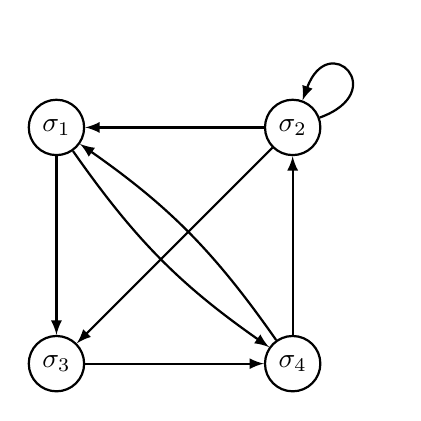
\begin{tikzpicture}[x=3cm, y=3cm]
\vertex (ul) at (0,1) {$\sigma_1$};
\vertex (ur) at (1,1) {$\sigma_2$};
\vertex (ll) at (0,0) {$\sigma_3$};
\vertex (lr) at (1,0) {$\sigma_4$};
\draw [->,thick] 
(ur) edge (ul)
(ul) edge (ll)
(ll) edge (lr)
(lr) edge (ur)
(ur) edge (ll)
(lr) edge[bend right=10] (ul)
(ul) edge[bend right=10] (lr);
\draw [->,thick] (ur) to [out=20,in=70,looseness=8] (ur);
\end{tikzpicture}	
\end{flushright}

\end{subfigure}
\begin{subfigure}{0.7\textwidth}
\begin{align}
f_1(\sigma_2,\sigma_4) & = |\sigma_2 \lor \sigma_4| = 1-(1-|\sigma_2|)(1-|\sigma_4|),\\
f_2(\sigma_2,\sigma_4) & = |\sigma_2 \rightarrow \sigma_4| = 1-|\sigma_2|(1-|\sigma_4|),\\
f_3(\sigma_1,\sigma_2) & = |\lnot \sigma_2| = 1 - |\sigma_2|,\\
f_4(\sigma_1,\sigma_3) & = |\sigma_1 \oplus \sigma_3| = |\sigma_1|(1-|\sigma_3|)+(1-|\sigma_1|)|\sigma_3|.
\end{align}
\end{subfigure}
\end{figure}


\paragraph*{}
The adjacency matrix of this graph is:
\begin{equation}
A =
\begin{bmatrix}
0 & 1 & 0 & 1 \\
0 & 1 & 0 & 1 \\
1 & 1 & 0 & 0 \\
1 & 0 & 1 & 0
\end{bmatrix}
\end{equation}

\paragraph*{}
One of the first things we notice is that loops in the graph are possible. Thus the function $f_2$ depends on the value of $\sigma_2$. Another thing is that even though $f_3$ is said to be a function of the variables $\sigma_1$ and $\sigma_2$, it depends only on $\sigma_2$.  So we could remove the edge $e_{31}$ and the dynamics of the whole system would remain the same. Let us consider this example a little bit further and see what else we can learn from it. We start by initializing the variables with values and choose them to be all zero. We can write this as a string in the form of $|\sigma_4||\sigma_3||\sigma_2||\sigma_1|$, which would be in our case $0000$. To calculate the next time-step, one goes through all the functions:
\begin{align}
f_1(0,0) & = 1-(1-0)(1-0) = 0,\\
f_2(0,0) & = 1-0\cdot(1-0) = 1,\\
f_3(0,0) & = 1 - 0 = 1,\\
f_4(0,0) & = 0\cdot(1-0)+(1-0)\cdot 0 = 0.
\end{align}

\paragraph*{}
Notice that even though $f_2$ would have changed the value of $\sigma_2$, we used its old one for $f_3$. This way of updating the state is called synchronous because all the functions are calculated simultaneously. We will always do it like this. Another possibility would be to pick one vertex randomly at a time and only update its variable. It would be the asynchronous method, but this is not of our interest from here on, since the system would no longer be deterministic.
After the update, the new string reads $0110$ or as its integer representation $6$, if we interpret it as a binary number.\footnote{Converting a binary string $n_N\cdots n_1$, with $n_i\in\{0,1\}$ for all $i\in\{1,\dots,N\}$ into decimal can straightforward be calculated as the sum $\sum\limits_{i = 0}^N n_i 2^i$.} Continuing with the update process over and over again creates the following chain:
\begin{equation}\label{eq:cycle3}
0 \rightarrow 6 \rightarrow 9 \rightarrow 15 \rightarrow 3 \rightarrow 9 \rightarrow 15 \rightarrow 3 \rightarrow 9 \rightarrow \dots\ .
\end{equation}

\paragraph*{}
After some steps, the states start to repeat themselves and will not leave the arrived cycle anymore. Thus one would now go ahead and initialize the system ones again, preferably with a state that we did not already have in the path above. The next unvisited integer value would be $1$ and if we start with it, we get:
\begin{equation}\label{eq:cycle1}
1 \rightarrow 14 \rightarrow 11 \rightarrow 11 \rightarrow 11 \dots\ .
\end{equation}

\paragraph*{}
Applying the update rule to the state $11$ leads again to itself. Thus when we compare it with the definition in equation (\ref{eq:fixpoint}), we can conclude that we found a fixpoint. All this means we have at least two separate paths that will never cross each other. If one goes through all other states, they would either lead to the cycle in equation (\ref{eq:cycle3}) or the fixpoint in equation (\ref{eq:cycle1}). What does this tell us now about the dynamics of a BN?

\paragraph*{}
Remember that the collection of all possible states the network can be in is the phase space. For a BN of size $ N $, there are exactly $ \Omega = 2^N $ different states. In the example, this would have been $16$. When a system with only a finite-sized phase space evolves over time, it will inevitably come to a state it already has been in and thereon repeating the path up to itself again on a cycle. The number of states a cycle contains is called its length and will be denoted by $ L $. 

\paragraph*{Attractors}
We now call an attractor a cycle that can be reached from states that are not part of itself, analogous to a contracting phase space of continuous dynamical systems. Since finding a cycle that is not also an attractor is pretty rare, we will not distinguish between the two. Attractors of length $ L=1 $ are also often referred to as fixpoints. All states that lead to an attractor plus its cycle elements are called the basin of attraction. We denote its number by $ \mathcal{N}_B $. In the literature, those are also called modules, as in \cite{aldana2003boolean}. All in all, this means that we have found in the example network two different attractors with lengths $3$ and $1$.

\begin{figure}[t]
	\centering
	\includegraphics[width=0.7\textwidth]{Plots/phase_space}
	\par
	\vspace{0.3cm}
	\caption{This figure is the schematic representation of a finite-sized phase space of any time-discrete and deterministic system. Every circle is a possible state $ \Sigma $ in phase space. The arrows go to the next state to which the current step leads after a single time step. Here the system has three attractors, sometimes also called modules in the literature. The red circles are states of their so-called cycles, which will repeat themselves over and over again. On the left side is an attractor with five red states. Thus it is said to have a length $ L $ of five. In light green, we have the garden-of-Eden states and all states that lead to the same cycle, plus its states themselves are the basin of attraction.}
	\label{fig:phase_space}
\end{figure}

\paragraph*{Garden-of-Eden States}\label{sec:garden-of-Eden}
A state without predecessor is called garden-of-Eden state. The G-density $\Gamma$ is defined as the fraction those $\mathcal{N}_G$ states are compared to the whole basin of an attractor. A precise definition could not be found throughout the literature, so that we will define it using the following equation:
\begin{equation}\label{eq:g-density}
\Gamma = \left\langle\tfrac{\mathcal{N}_{G}}{\mathcal{N}_{B}}\right\rangle_{\text{Attractors}}.
\end{equation}
So we take the average over all attractors in the system, which is a nice way of doing it generalizes to the case when we have finally introduced random Boolean networks. For a graphical representation of all the previously introduced concepts, see Figure \ref{fig:phase_space}.

\section{Random Boolean Network Ensembles}

\paragraph*{}
This thesis is mainly about the random Boolean network (RBN) model introduced by S. Kauffman in 1969 \cite{kauffman1969homeostasis} and in this section, we will finally introduce the final ideas necessary to comprehend our work. The arguments and derivations here and in the following chapter will mainly follow three sources. The first one to mention is the review from M. Aldana et al. \cite{aldana2003boolean} in which they highlighted the aspects of cycle behavior and information flow in such systems. Secondly, we used the review by B. Drossel \cite{drossel2008random}, from which we gained insights on RBNs up to the level of individual node behavior. And not at least to mention as source the book of C. Gros, in which he gave a broad overview of the topic and comprehensively derived specific properties. Whenever we use something of them or other authors almost one to one, this will be stated explicitly. But for all other cases and to provide a good reading flow, we will refer to them as our primary sources.

\paragraph*{}
One of the main differences to what we have described in the previous section is that we will move away from looking at individual networks and describe fairly large ensembles. Also, until now, there was no randomness involved in all our definitions. So, where does this come into play with RBNs? Exactly twofold: graph structure and choice of Boolean functions.

\paragraph*{Out-degree Distribution}
We are mainly interested in the $ N $-$ K $-Network model, how S. Kauffman defined it in 1969 \cite{kauffman1969metabolic}. In his honor, those networks often are referred to as Kauffman-Networks.  Those are Boolean networks with $ N $ vertices, where each of those has an in-degree of $ k^{(in)} = K $, with a constant $ K \in \{1,\dots,N\} $. Thus, every variable depends on the values of $ K $ randomly chosen nodes. We can calculate the probability distribution of the out-degree $ p_{k}^{(out)} $ as a Bernoulli process. We pick for every node two other ones, so the likelihood of choosing a certain vertex becomes $ p = K/N $. This random choice gets repeated for every node. Thus the probability of having an out-degree of $ k $ becomes:
\begin{equation}\label{eq:Poisson}
p_{k}^{(out)} = {N\choose k}p^k (1-p)^{N-k}\ \ \stackrel{1\ll N}{\longrightarrow}\ \ \frac{K^k e^{-z}}{k!}.
\end{equation}

\paragraph*{}
This is just the Bernoulli process, for which we defined the probability in equation (\ref{eq:Bernoulli}). The right side is an approximation for very large $ N $. This is the so-called Poisson distribution and it can be derived like C. Gros \cite{gros2010complex} showed it in his book in the chapter on graph theory. Suppose we have a very large $ N $, from which immediately follows a small $p=\tfrac{K}{N}$. Then the following approximations can be made and thereby also the one in equation (\ref{eq:Poisson}) holds for all finite node degrees $ k $:
\begin{equation}
{N\choose K} = \frac{N!}{k!(N-k)!} \simeq \frac{N^k}{k!},\ \ \ \ \left(1-\frac{K}{N} \right)^N \simeq e^{-K},\ \ \ \ \left(1-\frac{K}{N} \right)^{-k} \simeq 1.
\end{equation}

\paragraph*{}
Of course, one could also go the other way around and construct a given out-degree distribution network. Like R. Serra et al. did, there works \cite{serra2004dynamics} and \cite{serra2008simulation} for a scale-free topology. The distribution for this would be of the form
\begin{equation}\label{eq:scale_free_degree_distribution}
p_k^{(out)} = \frac{1}{\zeta(\gamma)}k^{-\gamma}\text{, with } \zeta(\gamma)= \sum\limits_{k=1}^{k_{max}}k^{-\gamma}.
\end{equation}

\paragraph*{}
Since we allow self-coupling, it would be $k_{max}=N$. Thus, for $N\longrightarrow \infty$ the $\zeta(\gamma)$ is just the Riemann-zeta function. In the exponent, we have the so-called scaling parameter $\gamma$ that is as far as we are interested, just a real value greater than one. Now you would construct a graph that obeys this distribution. We will not discuss how this would have to be done, since this is more of a side note. There are reasons one could choose such a topology over what we have described before, which could come from observations in the natural world. But since we are more interested in the model, we will stick to the way that constructs networks most randomly. In fact, if you consider large enough ensembles, they will contain all kinds of different topologies. As such, the scale-free networks are also part of our studies. We simply do not favor them over others. Another thing would be to vary the in-degree of the network, which we will have to do when the average degree $K$ is not an integer.

\paragraph*{Coupling Functions}
There are a couple of ways to decide on the coupling functions, once the network structure has been determined. We will here just present them in a similar fashion to the one of B. Drossel \cite{drossel2008random} in her review:
\begin{itemize}
	\item[-] Magnetization bias: We introduce the probability $p$ with which we choose a $ 1 $ as the output of the function for a given set of input values. With two input variables, for example, the implication $\sigma_i \rightarrow \sigma_j$ would then appear with the probability $ p^3(1-p) $, since it becomes only $0$ when $\sigma_i = 1$ and $\sigma_j = 0$. Generally speaking, if a function has $M$ outcomes with probability $ p^n (1-p) ^{M-n} $, we would pick a function with $ n $ ones. The most equally distributed choice and the one S. Kauffman used to introduce the model would be $ p=0.5 $.
	\item[-] Weighted classes: When we divide the possible binary functions into different classes as we did for two variables in section \ref{sec:binary_logic}, we can introduce weights for each class, with which we will take one of this class. For $n$ different classes, we pick the weights $ w_1 \dots w_n $ for every one of them. As they must be proper weights, they fulfill $ \sum w_i =1 $ and all of them are $w_i \in [0,1]$. The weighted method could be useful when someone finds that natural networks tend to prefer a certain class of functions. As seems to be the case with gene regulatory networks, which tend to be more often canalizing functions, see \cite{harris2002model} or \cite{kauffman2003random}. 
\item[-] Threshold functions: We could be interested in modeling some properties of firing neurons and therefore decide to use functions that only activate if enough input states are active. We then define the function for the $i$-th vertex with $ n $ in-going edges as:
\begin{equation}
f(\sigma_{i_1},\dots , \sigma_{i_n}) = \begin{cases}
1 &\text{if } \sum\limits_{j=1}^{n}\sigma_{i_j}>h,\\
0 &\text{else},
\end{cases}
\end{equation}
	where $ h $ would be a threshold greater than zero.
	\item[-] Cellular automaton with random couplings: We assign to every vertex the same coupling function.
\end{itemize}

\paragraph*{}
As before with the topology decision, all other cases would be interesting to study on their own, but the focus of our attention will be the magnetization bias method.

\paragraph*{Number of possible RBNs}
I. Harvey and T. Bossomaier \cite{harvey1997time} estimated the number of all possible RBNs with $N$ vertices and the in-degree $ K $ in the following way. You have to choose $ K $ other nodes for one of them, leading to $ N!/\left[K!(N-K)!\right]  $ possible ways of doing this. Then there are $ 2^{2^K} $ possible coupling functions, as we explained in section \ref{sec:binary_logic}. Since this has to be done for all $ N $ vertices, it is clear that the number of all possibilities becomes 
\begin{equation}
\left[2^{2^K}{N\choose K}\right]^N .
\end{equation}

\paragraph*{}
This entails even for fairly small networks a huge amount of possibilities. For example, say we have $N = 4$ and $K = 2$, leading to a number of $8.49\cdot 10^7$ rounded. Of course, one could argue that this estimation is a little bit far fetched. If you have a given network and change the outcome for every boolean function from $0$ to $1$ and the other way around, you may have a different network. But from a dynamical point of view, their behavior is identical. Another argument for a smaller estimate would be that there is no difference between the nodes. Thus there will be topologically equivalent networks. Both of these points would reduce the total count of different networks by some amount. But for all practical purposes, this is irrelevant since there is no practical way of determining whether a network is in principle the same in a somewhat large ensemble of them yet.

\paragraph{Ensambles, Mean Values and Variance}
An ensemble is a collection of several randomly initialized network realizations. More precisely, we will work most of the time with ensemble averages. If we are interested in some value, like the number of attractors $ \mathcal{N}_A $ in the RBNs of a certain kind, we store their values in a set $\mathcal{S}$. With $|\mathcal{S}|$ realizations, we will get the values $\mathcal{N}_A^{(1)},\dots,\mathcal{N}_A^{(|\mathcal{S}|)}$ and can take their ensemble average as:
\begin{equation}
\langle \mathcal{N}_A \rangle := \langle \mathcal{N}_A \rangle_\mathcal{S} := \frac{1}{|\mathcal{S}|} \sum\limits_{i=1}^{|\mathcal{S}|} \mathcal{N}_A^{(i)}.
\end{equation}
Whenever it is clear on which set the average gets taken, we can omit to write it down besides the right angle. The variance is a measure on how much the individual found values differ from this average, thus it is defined as:
\begin{equation}
\sigma^2 = \langle (\mathcal{N}_A-\langle \mathcal{N}_A \rangle)^2 \rangle.
\end{equation}
Taking the squareroot of this gives us the so-called standard deviation $ \sigma $.

\paragraph*{Hamming Distance}
The Hamming distance is a tool for measuring differences between two strings of information of equal length. For two states $ \Sigma $ and $ \tilde{\Sigma} $ it is defined as:
\begin{equation}\label{eq:hamming_distance}
D(t) = \sum\limits_{i = 1}^N \left( \sigma_i(t) - \tilde{\sigma}_i(t) \right)^2.
\end{equation}
For RBNs, we need it in order to measure how much information the system preserves over time. If we consider this to be a distance, we can ask ourselves if it will grow over time for two close, but not identical, initial states.

\paragraph*{}
We could define many more things concerning the dynamics of RBNs right now, but they seem to be more fitting in the context of our research. Thus, we will introduce them in the next chapter, when they actually appear to be needed. By now, we should have gained a clear picture of the model we are using and all the necessary mathematical background it was built on.

\paragraph*{Ergodic Sets}\label{sec:ergodic_set}
Ergodic sets were already proposed in 1969 by S. Kauffman himself, who thought them to be a good candidate for representing different cell types \cite{kauffman1969metabolic}. They are defined as the transition network that gets created by flipping single nodes in an attractor and connecting two of them, if such a change leads from the first ones cycle to the second. By now we know, that they themselves are not as useful as they were suspected to be for representing cell types, since most networks appear to have only a single ergodic set, like A. Ribeiro and S. Kauffman himself elaborated in \cite{ribeiro2007noisy}. 

\paragraph*{}
Ergodic sets are closely related to the topic of attractor robustness at which we also look in our work though we will prefer the name attractor stability for it. The robustness has often been of interest in studying random Boolean networks and can, for example, be found in works from B. Luque et al. \cite{luque1998stable}, or K. Willadsen et al. \cite{willadsen2008understanding}. We will later introduce the certain notion of attractor stability in which we are interested in.

\newpage\thispagestyle{empty}

\chapter{Methods and Results}\thispagestyle{fancy}
\paragraph*{}
Now we are equipped sufficiently to go deeper into our main topic of random Boolean networks and, more precisely, some statistical observations of their attractors and their stability behavior. Even though the previous chapter was said to be the theoretical background, we will onwards from here still encounter many theoretical aspects and derivations. In scientific research, there is no strict division between theory and observation. It is more like an interplay between those two aspects, as it has also been for us and the random Boolean networks the case.


\paragraph*{}
Random boolean networks (RBN) are discrete models where such attractors appear and due to their finitely large state space can accessibly be studied. They were first proposed by C. C. Walker and William Ross Ashby in 1966 \cite{walker1966temporal}, but got popularized by Stuart A. Kauffmans work in 1969, who wanted to model and understand gene regulatory networks \cite{kauffman1969homeostasis}. Over the years boolean networks have been used to model a wide variety of complex systems and their dynamics from many different fields such as social systems \cite{moreira2004efficient}, neural networks \cite{rosen2001multilayer} and the previously mentioned gene regulatory networks.

\paragraph*{}
All kinds of different models have been proposed and studied over time, e.g. using a certain type of network structure like in \cite{aldana2003boolean2}, \cite{iguchi2007boolean} and \cite{serra2004dynamics}, where they used scale-free degree distributions or choosing only canalizing coupling functions like in \cite{moreira2005canalizing}. Real gene regulatory networks have been showing some evidence for both approaches being reasonable (see \cite{moreira2005canalizing} and \cite{shaw2003evidence}).

\paragraph*{}
Since our main research interest lies in understanding the properties of attractors as such and not only compared to gene regulatory networks, we will stick to the classically proposed Kauffman-Network as our RBN. To avoid uncertainties we define our model in the following subsection and explain all necessary terms.


\section{Topological Properties}

\paragraph{}
Before starting investigations on any computational model, one has to make sure that the own implementations are correct and reproduce some already known properties. So we started by generating a few Kauffman-Networks and looked at their out-degree as our random variable $X=k^{(out)}$. The Poisson approximation presented in equation (\ref{eq:Poisson}) was what we were interested in checking first and it appears to be fairly good. It becomes even better for larger $N$ and smaller $ p = K/N $ as can be seen in Figure \ref{fig:Poisson}. 

\begin{figure}
	\includegraphics[width=\textwidth]{Plots/poisson_distributed}
	\caption{Three randomly created Kauffman-Networks with differing $N$ and $K$. The gray bars show the ratio the nodes with an out-degree of $k$ had compared to all others. The Poisson approximation (red, equation (\ref{eq:Poisson})) is a little off for the network on the right. But for the other two it appears to be pretty good.}
	\label{fig:Poisson}
\end{figure}

\paragraph*{}
The in-degree is due to the definition of the Kauffman-Network always $k^{(in)}=K$. Via the construction of choosing $K$ different nodes for every single node, this is guaranteed to be the case. 

\paragraph*{}
We started our studies of random boolean networks by recreating some known results to make sure our implementations work just as expected. Therefore we created networks with $N$ vertices and edges that would result in a constant $K=k^{(in)}$ and a Poisson distributed $k^{(out)}$. The results of our first attempts can be seen in Figure \ref{fig:phase_behavior} and recreate the long term behavior of RBNs in terms of their ability to propagate information in their different phases or instead how differences between states grow over time. We will explain this in the following in much more detail.

\section{Dynamics and Phases}
\paragraph*{}
Random Boolean Networks exhibit different behavior depending on the graph structure that is used. From the viewpoint of information flow, they can either retain or lose memory. The easiest way to see this is with a mean-field approximation of the $N $-$K $ model with magnetization bias $p$. It means we will not look at individual node behavior and instead focus on averages over the whole system. For this, we will always assume a large number of vertices $N\longrightarrow\infty$ in this section.

\paragraph{Mean-Field Approximation}
Let us say we have two different initial conditions $\Sigma_0$ and $\tilde{\Sigma}_0$. Their Hamming distance $D(0)$ can be calculated accordingly to equation (\ref{eq:hamming_distance}) and gives the number of elements that are different in these two states. A single node influences averagely $K$ other ones, thus $KD(0)$ coupling functions get affected in the next time step. There are two possible ways of having them be different, each with a probability of $p(1-p)$. In total this means that for the next time step the distance grows as $D(1) = 2p(1-p)KD(0)$. After the time $t$ it will recursively become:
\begin{equation}
D(t) = \left[2p(1-p)K\right]^t D(0) = D(0)e^{t\ln[2p(1-p)K]}.
\end{equation}
There are now three different things that can happen with such an equation. It can grow exponentially, go to zero or stay just the same, which happens if 
\begin{equation}\label{eq:critical_condition}
2p(1-p)K=1.
\end{equation}
Thus for a given magnetization bias $p$, the tipping point, where the system changes its behavior, also just called its critical connectivity, is at 
\begin{equation}\label{eq:critical_connectivity}
K_c = \frac{1}{2p(1-p)}.
\end{equation}
\paragraph*{}
Also, the other way around, if we fix $ K $ the critical bias for the coupling functions can be calculated by:
\begin{equation}\label{eq:critical_magnetization_bias}
p_c^{\pm}=\frac{1}{2}\pm \sqrt{\frac{1}{4}-\frac{1}{2K}}.
\end{equation}

\begin{figure}
	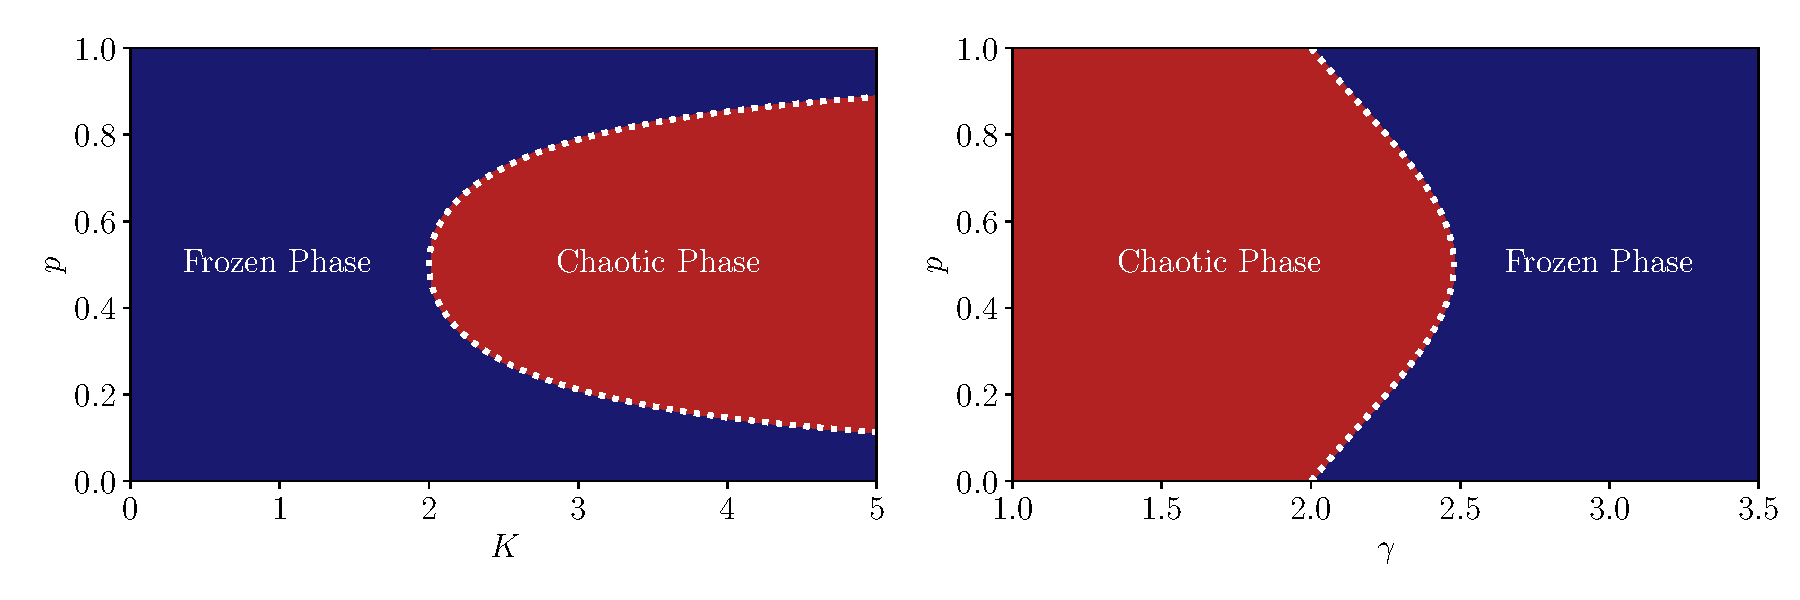
\includegraphics[width=\textwidth]{Plots/network_phases}
	\caption{Here we have the phase diagrams of different RBN models, with the magnetization bias $p$. Left: $N$-$K$ model, where the second parameter is the connectivity $K$. Right: Scale-free model, with the scaling parameter $\gamma$. }
	\label{fig:network_phases}
\end{figure}


\paragraph{}
In the context of the RBN, this means we have the following different phases:
\begin{itemize}
	\item[-] Frozen ($K<K_c$): The Hamming distance decreases over time and the two initially different states will most likely end up in the same configuration. It often coincides with the arrival at a fixpoint, which means the nodes stop changing over time, which is why this phase is called frozen. This means we lose all the initial information on the systems we had at the beginning over time.
	\item[-] Critical ($K=K_c$): At this point, the distance stays roughly the same according to the mean-field approximation. But since it only works on averages, the system's fluctuations at the critical value are not considered.
	\item[-] Chaotic ($K>K_c$): The different initial conditions diverge exponentially over time. Of course, with only a finite number of nodes $ N $, the difference between the two initial configurations can never get any larger than this. Thus, at every time step $t$, it will be $D(t) \leq N $, which is again something that the mean-field approximation does not account for.
\end{itemize}

\paragraph{}
Since we arrived at the critical condition in equation (\ref{eq:critical_condition}) only by looking at averages, the same argumentation also holds for scale-free networks. We only need to calculate the average out-degree and can do this by using the probability distribution given in equation (\ref{eq:scale_free_degree_distribution}):
\begin{equation}
K = \langle k^{(out)}\rangle = \sum\limits_{k=1}^{\infty}kp_k^{(out)} = \frac{1}{\zeta(\gamma)}\sum\limits_{k=1}^{\infty}k^{1-\gamma} =
\begin{cases}
	\infty                                & \text{if } 1 < \gamma \leq 2, \\
	\frac{\zeta(\gamma-1)}{\zeta(\gamma)} & \text{if } 2 < \gamma .
\end{cases}
\end{equation}

\paragraph*{}
Now we can solve for the critical magnetization bias with equation (\ref{eq:critical_magnetization_bias}). With this, we can create the transition curve of the phase diagrams for the $N$-$K$ model and scale-free networks, which we can see in Figure \ref{fig:network_phases}.

\paragraph*{}
\begin{figure}
	\begin{subfigure}{\textwidth}
		\includegraphics[width=\textwidth]{Plots/phase_behavior}
		\label{fig:sfig1.1}
	\end{subfigure}
	\caption{Here we reproduced some known classical results, as Aldana et al. have shown in their review \cite{aldana2003boolean2}. Both graphs show the normalized Hamming distance with respect to time for networks with $ N=10000 $ and $ K=4 $. The left is for the $ N $-$ K $ model and the right is for a square lattice with periodic boundary conditions. The simulation started at a random state and used as the comparison state the same one with $ 100 $ nodes flipped. We varied the bias between values from $ p_1 = 0.05 $ to $ p_10 = 0.275 $ and averaged for every one of them over $ 1000 $ network realizations.}
	\label{fig:phase_behavior}
\end{figure}

\paragraph*{}
We ran some simulations and measured the normalized Hamming distance for two states of the $N$-$K$ model and square lattice networks, which started with $1\%$ of their node values being different. The results can be seen in Figure \ref{fig:phase_behavior}. We got the idea for doing this from the work of M. Aldana et al. \cite{aldana2003boolean2}, though there can be found many other authors throughout the literature that also already did the same.

\paragraph*{}
The $N$-$K$ model is the one that shows the behavior we described just above. In the chaotic phase, the differences between the two states grow over time. Near the critical line at $ p_c = \tfrac{\sqrt{2}-1}{2\sqrt{2}} \simeq 0.1464 $ the amount of flipped vertices stays roughly the same. For networks in the frozen phase, the overwhelming majority of states tend to evolve into the same fixpoint and this only in a few steps.

\paragraph*{}
The square lattice networks, on the other hand, show somewhat different behavior. M. Aldana et al. \cite{aldana2003boolean2} give a value for the critical bias of around $p_c\approx 0.27$. However, as we can clearly see, the distance already retains or even grows with time for much smaller values. Moreover, the window from smallest to greatest bias is much more narrow to what we have seen before by direct comparison. This has to do with the high order of symmetry the underlying network possesses. The main takeaway from this could be that the underlying graph plays a significant role in random boolean networks' behavior.

\paragraph*{Annealed Approximation}\label{sec:annealed_approximation}
The previous mean-field approximation already delivered some exciting results, which are also in agreement with computational observations. But the argumentation appears to be quite rough and, as we mentioned above, can not account for any fluctuations in the system. Thus, we will look at another approximation, which can be done a little more rigorously and provides methods to observe additional properties.

\paragraph*{}
B. Derrida and Y. Pomea \cite{derrida1986random} presented in 1985 a new way to calculate several quantities of random boolean networks, which they called the annealed approximation. The name is an analogy from the field of spin glasses, where it means that certain random variables of the system can change over time. In the same language, all the models we have presented so far would be quenched since once we decided on the network structure and the boolean functions, those become permanent. In contrast to this, they can change at every time step in the annealed approximation. By this, they lose their correlation to the previously given boolean functions. The system also becomes non-deterministic and thereby, no attractors or related structured will appear any longer. But for large enough systems, where $N\longrightarrow\infty$, they will only play a secondary role anyway.

\paragraph*{}
The derivations we are making here are in the spirit of the original work from B. Derrida and Y. Pomea. We start again by considering two random different initial states $\Sigma_0$ and $\tilde{\Sigma}_0$ for a given random boolean network, that have a Hamming distance of $D(0) = n > 0$. The system has a large number of nodes $N$ and the coupling constant $K$. The nodes can be divided into two sets, the ones that are different $A$ and those that are the same in both states $B$. Only if a node takes input nodes from set $B$ it can have a different outcome for its value in $\Sigma_1$ and $\tilde{\Sigma}_1$. We now want to consider the odds that $N_0$ nodes only take their inputs from $A$. The probability for a single vertex to draw $K$ times only from $A$ is:
\begin{equation}\label{eq:draw_from_one_set}
q = \prod\limits_{i = 0}^{K-1}\frac{N-n-i}{N-i} \approx \left(\frac{N-n}{N}\right)^K.
\end{equation}
The right hand side is a good approximation for very large $N$ and only finitely large $K$. With this, we see that this is again a Bernoulli process and with equation (\ref{eq:Bernoulli}) we can calculate the probability distribution for $N_0$ to be:
\begin{equation}
Q(N_0) = {N \choose N_0} \left[\left(\frac{N-n}{N}\right)^K\right]^{N_0}  \left[1-\left(\frac{N-n}{N}\right)^K\right]^{N-N_0}.
\end{equation}

\paragraph*{}
If the nodes do take input from set $B$, the probability that they will be different in the next time step will be again $2p(1-p)$. This is all we needed to calculate the likelihood that we will have $m$ different nodes after a single time step:
\begin{equation}
\begin{split}
P_1(m) &= \sum\limits_{N_0 = 0}^{N-m} {N-N_0 \choose m} Q(N_0) \tilde{p}^m (1-\tilde{p})^{N-N_0-m} \\
&= \sum\limits_{N_0 = 0}^{N-m} \frac{(N-N_0)!}{m!(N-N_0-m)!}\frac{N!}{N_0 !(N-N_0)!} q^{N_0}  (1-q)^{N-N_0} \tilde{p}^m (1-\tilde{p})^{N-N_0-m}\\
&= {N \choose m} \left[\tilde{p}(1-q)\right]^m \cdot\sum\limits_{N_0 = 0}^{N-m} {N-m \choose N_0} q^{N_0}  \left[(1-q) (1-\tilde{p})\right]^{N-m-N_0}\\
&= {N \choose m} \left[\tilde{p}(1-q)\right]^m \left[1-\tilde{p}(1-q)\right]^{N-m}.
\end{split}
\end{equation}
This is a very nice result since it shows us that we have, in fact, again a binomial distribution with the individual probability of a single event to occur of $\tilde{p}(1-q)$. We could have also guessed that this must be the case since this is nothing else than the probability for a single node to be chosen from the set of nodes with unequal values and, at the same time, having functions that provide different outcomes. Nonetheless, it is good to see that after a short derivation, we end up with a clean and intuitive result. In their work, B. Derrida and Y. Pomea arrive at this equation in a way where it is not immediately apparent that this is just a binomial distribution.

\paragraph*{}
Now we know from section \ref{sec:bernoulli_process} that the expected value will just be $E[X] = N\tilde{p}(1-q)$, if $X$ is the random variable representing all possible values of $m$. The standard deviation is, as we know, proportional to $ \sqrt{N} $, which is neglectable compared to the whole possible range of $ X $, since
\begin{equation}
\frac{\sqrt{N}}{N} \stackrel{N\rightarrow\infty}{\longrightarrow}0.
\end{equation}
We can conclude that the peak around the mean is incredibly narrow compared to all possible values and because of this, it will be almost surely: $m = N\tilde{p}(1-q)$. Introducing the variables $y_0:=n/N$ and $y_1:=m/N$ and resubstituting $\tilde{p}$ and $q$ lets us rewrite the equation into:
\begin{equation}\label{eq:first_map}
y_1 = 2p(1-p)[1-(1-y_0)^K]
\end{equation}

\paragraph*{}
As of right now, we would not have needed to introduce the annealed approximation since all our arguments are also valid in the quenched model. But this changes if we have to consider the next time step and all others after that up to $t$. To redo the equation's derivation (\ref{eq:first_map}) we would have to respect the correlations to the first chosen functions. But in the annealed model, every step stays the same as before and we arrive at:
\begin{equation}\label{eq:annealed_map}
y_{t+1} = 2p(1-p)[1-(1-y_t)^K] =: \phi(y_t).
\end{equation}

\paragraph*{}
It is obvious that $y^* = 0$ is a fixpoint of this map and by calculating the derivative at it, we will analyze its stability:
\begin{equation}
\phi'(0) = 2p(1-p)K
\begin{cases}
\leq 1 & \text{if } K \leq K_c, \\
> 1 & \text{if } K > K_c.
\end{cases}
\end{equation}

\paragraph*{}
The critical connectivity is the same as we had before in equation (\ref{eq:critical_connectivity}). We see that for values greater than $K_c$, zero becomes an unstable fixpoint. This is what we conclude when comparing the results with the definition of fixpoint stability in equation (\ref{eq:fixpoint_stability}). We arrive at the same result as we had in the mean-field approximation and observe a change of behavior for systems that cross $K_c$. In addition to that, we now have the map (\ref{eq:annealed_map}) from which we can deduce complementary information on networks, where we know their average connectivity $K$. Let us define the random variable $Y$ as the normalized distance between two consecutive time-steps. The expected value of it should now be in agreement with the stable fixpoint of $\phi$ and it certainly is in the chaotic phase, which we can see in Table \ref{tab:fixpoints}.

\paragraph*{}
\begin{table}[h!]
	\centering
\begin{tabular}{|c|C{1.5cm}|C{1.5cm}|C{1.5cm}|C{1.5cm}|}
	\hline
	\multicolumn{5}{|c|}{$N=10^3$, Ensemble Size: $10^4$,} \\ 
	\multicolumn{5}{|c|}{Measured between: $t_1 = 49$ and $t_2=50$} \\ 
	\hline
	$K$ & $p$ & $y^*$ & $E[Y]$ & $\text{Std}[Y]$ \\ 
	\hline\hline  
	\multirow{3}{*}{3} & $0.212$ & $0.002$ & $0.039$ & $0.035$ \\ 
	\cline{2-5}
	& $0.300$ & $0.223$ & $0.219$ & $0.034$ \\ 
	\cline{2-5}
	& $0.450$ & $0.345$ & $0.344$ & $0.024$ \\ 
	\hline\hline 
	\multirow{3}{*}{4} & $0.147$ & $0.002$ & $0.029$ & $0.027$ \\ 
	\cline{2-5} 
	& $0.300$ & $0.341$ & $0.340$ & $0.020$ \\ 
	\cline{2-5}
	& $0.450$ & $0.450$ & $0.450$ & $0.017$ \\ 
	\hline\hline  
	\multirow{3}{*}{5} & $0.113$ & $0.001$ & $0.024$ & $0.023$ \\ 
	\cline{2-5}
	& $0.300$ & $0.382$ & $0.382$ & $0.017$ \\ 
	\cline{2-5}
	& $0.450$ & $0.475$ & $0.475$ & $0.016$ \\ 
	\hline
\end{tabular} 
\vspace*{0.3cm}
\caption{The observed random variable $ Y $ is the change of the normalized Hamming distance (equation (\ref{eq:hamming_distance}) divided by $ N $) for an ensemble of $ 10^4 $ RBNs, each with $ 10^3 $ nodes and certain fixed $ K $'s and $ p $'s between the $ 49 $ and $ 50 $ time-step after a random initialization at $ t = 0 $. We calculated the expected value (\ref{eq:expected_value}) and the standard deviation (\ref{eq:standard_deviation}) for $ Y $, which we compare to the second fixpoint of the map (\ref{eq:annealed_map}).}
\label{tab:fixpoints}
\par
\end{table}

\paragraph*{}
We come to similar conclusions as B. Derrida and Y. Pomea did in their original work. The map in equation \ref{eq:annealed_map} gives a pretty useful description for networks in the chaotic regime, even though we derived it with the annealed approximation. Near the critical point, the results are not as close anymore.

\paragraph*{}
The approximation is good for understanding some aspects of random boolean networks, but not for all. It excludes by its definition the appearance of any attractors and is therefore not suited for studying everything related to them. However, we gained a good understanding of networks' behavior in their different phases and how small perturbations grow over time.

\section{Attractors}

\paragraph*{}
Now we come to one of the main subjects of investigations of this thesis. We were interested in finding out more about the basins of attraction of attractors and wanted to study their structure, sizes, and how this relates to the cycles' length. Moreover, we wanted to do this for systems in the different phases and compare them like this.

\paragraph*{}
To average over sufficiently large network ensembles, we had to develop an efficient way of fully analyzing the whole phase space of a single realization. There have already been ways to find the whole basin of attraction for a single already found cycle, like the one introduced by A. Wuensche \cite{wuensche1997attractor}. 

\paragraph*{}
However, one has to reverse engineer all the states a single state could arise from by checking all the possible input values for every node that would lead to the appropriate values. This assumes full knowledge of all boolean functions, which our solution does not. With our algorithm, we only need to know the next state for every single state in the phase space, making it more general and applicable to other models than random boolean networks. We basically have just to go through all the states once forwards and then backward and collect all the necessary information on the fly. The main idea for this stems from how list types are defined in the programming language $\texttt{C++}$. For more details on our algorithm, see the Appendix \ref{sec:algorithm}.

\paragraph*{}
\begin{figure}[t]
	\includegraphics[width=\textwidth]{Plots/basin_sizes_N14}
	\caption{Here we plotted attractor length $ L $ against the fraction the basin of attraction occupies compared to the whole phase space (normalized basin size). Those examples are representatives for the different phases of boolean networks. All their coupling functions have a bias of $ p = 0.5 $. Below those scatter plots, we see the probability distribution for a cycle to have length $ L $. The green triangles are the proportion of the phase space which are garden-of-Eden states. All ensembles were created over $ 10^6 $ network realizations and $ L_{max} $ is the longest attractor we could find in each of those sets.}
	\label{fig:basin_sizes_main}
\end{figure}

\paragraph*{}
Figure \ref{fig:basin_sizes_main} can be seen as a summary of some of our main findings. However, what we see in this graphic is far too rich and we will go through everything there is to notice in many more details in the following subsections. What can be obviously stated is that the size of the basins of attraction has wildly different behavior comparing networks in the frozen phase, on the critical line and in the chaotic phase.

\paragraph*{}
We can make a few remarks on the phases of random Boolean networks in general before we continue with the more detailed studies of the results. If you look at Figures \ref{fig:basin_sizes_main_additional_sizes} and \ref{fig:basin_sizes_main_additional_frozen_chaotic}, you can make the following two observations. First, the results we get for the averaged sizes of the basins of attraction are very similar for different network sizes. Here we only showed $N=10$ and $N=12$ as examples, but this is the case at least for networks between the sizes $N=6$ and $N=16$. For the larger networks, we created only fewer realizations. Thus we decided to only look at $N=14$ systems in Figure \ref{fig:basin_sizes_main} and not the larger ones.

\paragraph*{}
The second general observation we can make is that even though we can accurately calculate the critical values, the network ensembles' observed behavior seems to be rather gradually changing between similar connectivities $K$. If we look at an ensemble at sets with critical systems, it is not too hard to understand why we would find that it is like this. We use realizations where everything gets determined at the start with random probabilities. Thus we will have realizations that tend to be either in the frozen or chaotic phase, rather than only critical ones. 

\paragraph*{}
To construct an extreme case, we could think about a network, which got applied only with constant and fully canalizing coupling functions. Such a system is not too unlikely for smaller system sizes and is definitely one that belongs with its behavior to the frozen phase. Consider random couplings on top of the randomly chosen Boolean functions. Then, even for larger systems, there will also be a non-zero probability to create a realization that would rather belong to the frozen phase. Similarly, we could make this argument for systems that would rather belong in the chaotic phase.

\paragraph*{}
So, all in all, we have for $K=2$ a mixture of critical systems and those belonging to the frozen or chaotic phases. And depending on whether we choose coupling values below or above, we will get more of the one or the other in our ensemble data, which explains the gradual change between the values. 

\paragraph*{}
That criticality is still not only a mixture of frozen and chaotic systems can be seen by looking at the maximal lengths $L_{max}$ we could find in all three regions. They are longer in the chaotic phase than in the frozen one, which had to be expected. But the largest cycles we could find within ensembles of $10^6$ realizations happened for all system sizes to be around the critical value. There is no way to explain this observation with the previous explanation. Thus it means something special having critical RBNs, even if we do not look at them in the thermodynamical limit, at which we derive most notions of criticality in general.


\subsection{Garden-of-Eden States}
\paragraph*{}
Throughout the literature, one does not find too many works on the garden-of-Eden states, though they are regularly mentioned. One example would be the Ph. D. thesis of A. Wuensche \cite{wuensche1997attractor}, where he analyzed the G-density and the phase space in-degree for cellular automata (CA). Those are not the same as our RBNs, but they are closely related. One could say that CAs are basically RBNs with a grid structure as their network and every node gets applied with the same boolean function.

\paragraph*{}
\begin{figure}
	\includegraphics[width=\textwidth]{Plots/in_degree_N10}
	\centering
	\caption{Those are the in-degree distributions that we obtain by analyzing the state space of different network ensembles. For comparison, we draw on the right the distribution we get by randomly choosing the next time step out of all $2^{14}$ possible states.}
	\label{fig:in-degree}
\end{figure}

\paragraph*{}
We already introduced the concept of garden-of-Eden states in section \ref{sec:garden-of-Eden}, but in short such states are the ones that can only be reached through being an initial condition. When we look at Figure \ref{fig:basin_sizes_main} again, it becomes pretty obvious that the part the garden-of-Eden states take from the whole basin of attraction is pretty large. To put it more quantitatively, we ran simulations for different network sizes in all different phases and measured their G-densities $\Gamma$ (see equation (\ref{eq:g-density})):
\begin{table}[h!]
\centering\label{tab:g-density}
\begin{tabular}{|c|c|C{1.5cm}|C{1.5cm}||c|c|C{1.5cm}|C{1.5cm}|}
	\hline 
	\multicolumn{8}{|c|}{Ensemble Size: $10^6$}\\
	\hline
	$N$ & $K$ & $\Gamma$ & $\text{Std}(\Gamma)$ & $N$ & $K$ & $\Gamma$ & $\text{Std}(\Gamma)$  \\ 
	\hline \hline
	\multirow{3}{*}{8} & $1.5$ & $0.919$ & $0.067$ & \multirow{3}{*}{12} & $1.5$ & $0.979$& $0.022$\\ 
	\cline{2-4} \cline{6-8} 
	 & $2$ & $0.813$ & $0.122$ & & $2$ & $0.926$ & $0.060$ \\ 
	\cline{2-4} \cline{6-8} 
	 & $8$ & $0.325$ & $0.146$ & & $12$ & $0.337$ & $0.124$ \\ 
	\hline \hline
	\multirow{3}{*}{10} & $1.5$ & $0.959$ & $0.039$ & \multirow{3}{*}{14} & $1.5$ & $0.989$ & $0.013$ \\ 
	\cline{2-4} \cline{6-8} 
	& $2$ & $0.882$ & $0.087$ & & $2$ & $0.953$ & $0.041$ \\ 
	\cline{2-4} \cline{6-8} 
	& $10$ & $0.332$ & $0.133$ &  & $14$ & $0.341$ & $0.116$ \\ 
	\hline 
\end{tabular} 
\vspace*{0.3cm}
\caption{Here we measured the G-density (\ref{eq:g-density}) and its standard deviation (\ref{eq:standard_deviation}) for different network sizes in all phases.}
\par
\end{table}

\paragraph*{}
As we have already seen before, the garden-of-Eden states make up the greatest portion of the attraction basin in the frozen phase and on the critical line but are far less common for chaotic systems. Another thing to notice is the more nodes our system has, the greater the G-density seems to become. Thus, we might hypothesize that every randomly chosen initial condition in the thermodynamic limit will almost surely be a garden-of-Eden state, excluding chaotic systems.

\paragraph*{}
Now we want to know what makes the chaotic networks different from the other ones. Therefore it would be interesting to analyze the structure of the phase spaces even further. When we look again at Figure \ref{fig:phase_space} it is obvious how the structure of the phase space itself can be seen as a graph. And in it, the garden-of-Eden states are the ones that have an in-degree $k^{(in)}$ of zero. So the logical next step would be to look at different $k^{(in)}$s. In Figure \ref{fig:in-degree} we see the results of this. We also looked at the distribution for distributing $\Omega$ links over $\Omega$ nodes, which is simply a binomial distribution.

\paragraph*{}
We can observe that chaotic systems' in-degree distribution resembles more random ones than those in the frozen or critical ones. Especially in the $N=K$ case, we can explain this pretty well. Since every node has inputs from all other ones and itself, there are $2^N$ values to decide on for their coupling functions at the initialization. Or, to put it in other words: every state of the $2^N$ states in the phase space uniquely determines the next time step of every single node. Thus, from every point in time, the network's evolution can be viewed as flipping a coin for every variable. It just already happened at the initialization of the RBN. So at least for two consecutive time steps, this view makes the system's evolution in principle random and reminds us of how we introduced the annealed approximation. As was the case in this model, we ignored the long-term correlations of the functions, which is why the distribution, in the end, is not identical to that of a completely random one. But it is a good enough first approximation, with which we are satisfied.

\paragraph*{}
In contrast to the chaotic networks, explaining what we see for critical systems and frozen ones requires a little more thinking but is also not too complicated to grasp. We will try to make the behavior plausible for $K=2$ RBNs, but for the other ones, the reasoning is analogous. 

\paragraph*{}
First of all, what do the in-degree distributions tell us about the structure of the phase space? We see a very high number of garden-of-Eden states and some in-degree values relatively high compared to the random case. Thus, many different states lead to only a few ones, which dominate the network's dynamical behavior. To draw an analogy to the continuous dynamical system, one could say that the phase space contracts fast around the paths limiting the attractor cycles.

\paragraph*{}
So if you take a look at Table \ref{tab:two_dim_fun} again and remember the different classes, we can make sense of the observed. The first class $\mathcal{A}$ does not depend on the inputs at all and the classes $\mathcal{B}_1$ and $\mathcal{B}_2$ do only partially so. This means that once we evolved from an initial condition into our current state, it is very likely that there also exist several other states from which we could have come from. A fairly good understanding on this can be gained by looking at the work of B. Drossel \cite{drossel2008random}. Here she divides the nodes into three categories: the frozen core, the irrelevant ones and the relevant ones. 

\paragraph*{}
The frozen core is simply the vertices that do not change their value along their path. The irrelevant nodes do change over time, but they do not influence the values of other nodes. They are only on the receiving side and are basically a dead end on the flow of information. The remaining nodes are the relevant ones, those that are influenced by previous nodes and determine the values of the ones coming after them. Those are the ones that completely dominate the dynamical behavior of the networks. For the critical $K=2$ model, B. Drossel \cite{drossel2008random} shows an analytical derivation in her review with the result that the number of those is in the thermodynamic limit proportional to $N^{1/3}$. Moreover, the number of relevant nodes that receive inputs from two other relevant nodes stays finite even for infinitely large systems.

\paragraph*{}
In return, this means that only a number on the order of $2^{N^{1/3}}$ states is actually relevant for the system's dynamics. The other states of the phase state do not have this much importance and only lead up to those first ones. Thus, it is plausible that we have many states with zero and only a few with very high in-degrees.

\subsection{Chaotic Networks}
\paragraph*{}
On the right side of Figure \ref{fig:basin_sizes_main} we had in the lower plot the probability distribution of attractors with the length $L$. With the average number of cycles $\left\langle N_c(L) \right\rangle$ with length $L$, it could be calculated as:
\begin{equation}\label{eq:length_probability_raw}
P(L)=\left\langle N_c(L) \right\rangle  \left[\sum\limits_{l=1}^{\Omega} \left\langle N_c(l) \right\rangle\right]^{-1}.
\end{equation}

\paragraph*{}
Aldana et al. \cite{aldana2003boolean} presented a comprehensible derivation of $\left\langle N_c(L) \right\rangle$ in which they used the annealed approximation. C. Gros \cite{gros2010complex} goes through the individual steps in much more detail and we will follow his argumentation only with a little variation in where we use our Taylor expansion.

\paragraph*{}
In section \ref{sec:annealed_approximation} we were going through the annealed approximation in quite some detail. We were also pointing out that it would exclude the appearance of any attractors by its definition. This is true but can be changed by viewing the state space as large enough for us to treat it as infinite in our calculations while at the same time considering that it is actually finite for any real-world random Boolean network.

\paragraph*{}
Again, the system's path is basically a random walk, but now we will also consider that there exist only $\Omega$ states. We start with an easily computable value, namely the probability $p_{t+1}$ that after $t+1$ time steps, a cycle will not close. At that time, there is a fraction of $1-(t+1)/\Omega$ possible states left that will not close the loop. Additionally, we arrived at this point only if there happened no enclosing before, which happened with the probability of $p_t$. Together we get the following recursion relation:
\begin{equation}
p_{t+1} = p_t \left(1-\frac{t+1}{\Omega}\right).
\end{equation}

\paragraph*{}
It is impossible that a cycle closes at initialization and thus $p_0 = 1$ what we can immediately use:
\begin{equation}
\begin{split}
p_{t+1} &= p_t \left(1-\frac{t+1}{\Omega}\right)\\
&= p_0 \prod\limits_{i=1}^{t+1} \left(1-\frac{i}{\Omega}\right)\\
&= \prod\limits_{i=1}^{t+1} \left(1-\frac{i}{\Omega}\right).
\end{split}
\end{equation}

\paragraph*{}
\begin{figure}[t]
	\includegraphics[width=\textwidth]{Plots/chaotic_hist}
	\centering
	\caption{Here we brought equation (\ref{eq:number_cycles_chaotic}) into a form, where we can compare theory and simulation as the classically known parabola. On the right, we have the original distribution as we have already shown it in Figure \ref{fig:basin_sizes_main} on the right. We measured over $ 10^7 $ realizations and each bin contains minimally on the order of hundreds of attractors.}
	\label{fig:quadratic_average_number_of_cycles}
\end{figure}

\paragraph*{}
Now we can take the logarithm on both sides of the equation, which we then Taylor expand on the righthand side, assuming a large number of total possible states $\Omega$:
\begin{equation}
\begin{split}
\log{(p_{t+1})} &= \log{\left[\prod\limits_{i=1}^{t+1} \left(1-\frac{i}{\Omega}\right)\right]}\\
&= \sum\limits_{i=1}^{t+1} \log{\left(1-\frac{i}{\Omega}\right)}\\
&= \sum\limits_{i=1}^{t+1} \left[- \frac{i}{\Omega} + O\left(\frac{i^2}{\Omega^2}\right)\right]\\
&\approx - \frac{t(t+1)}{2\Omega}.
\end{split}
\end{equation}


\paragraph*{}
The last step was done by neglecting all the terms with omega of order two or higher in the denominator and summing over the natural numbers from $1$ to $t+1$. Now we can further approximate that the time we have arrived at is also large but, of course, still negligible compared to $\Omega$, because then we can rewrite $t(t+1)\approx t^2$. This is actually not necessary to do but makes further calculations easier and has also been done by the authors we follow in this derivation. Moreover, we will also assume that the cycle length we are interested in is also fairly large and we have $L-1\approx L \approx L+1$.

\paragraph*{}
Now we have all we needed to finally compute $\left\langle N_c(L) \right\rangle$. We get a cycle of length $L$ if the loop closes after exactly $L$ time steps and does so with the initial state. That this state gets chosen at random has the same probability as any other state and is, therefore, $\Omega^{-1}$. But since we could have started the path from any of the $\Omega$ states, those two values cancel each other out in the calculation. If we now take into account that by this procedure, every state of a single cycle increases the number of counted cycles by one and also do not forget that there should not be an enclosure for $L-1$ states, we finally arrive at:
\begin{equation}\label{eq:number_cycles_chaotic}
\left\langle N_c(L) \right\rangle = \frac{p_{L-1}}{L} = \frac{\exp{\left[-L^2/(2\Omega)\right]}}{L}.
\end{equation}

\paragraph*{}
With this result and equation (\ref{eq:length_probability_raw}) we could now compare the results from Figure \ref{fig:basin_sizes_main}. We did this in Figure \ref{fig:quadratic_average_number_of_cycles} but decided to bring the equation into a form where the curve is represented in a familiar form, namely a parabola. 

\paragraph*{}
We see that this relation holds in the chaotic phase quite well, even for relatively small system sizes. At first glance, this might seem surprising since we made a series of approximations on the way to the final result. Still, when we remind ourselves that the number of states is $\Omega=2^{N}$, it becomes clearer. We neglected terms of this value to quadratic order in the denominator inside an exponential function. Thus, we were basically already multiplying by a value really close to one.

\paragraph*{}
\begin{figure}[t]
	\includegraphics[width=\textwidth]{Plots/N_K_compare}
	\caption{Here we have put $K=N$ networks for the system sizes of $N=10, 12$ and $14$ alongside each other for comparison. We checked the average size of the basins of attraction against the length of the attractors' cycles. On the left, we did so without any rescaling and on the right, we rescaled the axes of the length with a factor of $1/\sqrt{2\Omega}$, which we have chosen because of equation (\ref{eq:number_cycles_chaotic}). This makes the curves more comparable and we see that for lower $L$, the curve starts steeper for larger system sizes. Still, for lengths round about $L\approx \sqrt{2\Omega}$ there is no real difference between the different ensembles anymore.}
	\label{fig:N_K_compare}
\end{figure}

\paragraph*{Sizes of the Basins of Attraction}
In Figure \ref{fig:basin_sizes_main}, the size of the basin of attraction is monotonically increasing with the length of an attractor. This is also very plausible when we again view the chaotic system in the annealed approximation. If we have a certain number of cycles and randomly link the remaining states to them, the longer ones will also have many incoming edges. 

\paragraph*{}
To come up with a good approximation seems to be an open problem and it is clear why that is the case. For a calculation, we would have to think about the cycle length and that the states that already lead to the attractor could then also be picked at random in the process. Furthermore, it is not enough to know the probability $P(L)$ of a cycle to have length $L$, but also the conditional probability $Q(S|L)$ of having additional cycles which lengths sum up to a certain value $S$. So, for now, this will have to stay an open problem.

\paragraph*{}
But there are still other things to look at and we can analyze the results of our simulations at least quantitatively. In Figure \ref{fig:N_K_compare}, we looked at the sizes of the basins of attraction for different system sizes. They all have similar behavior, which becomes even more apparent when we rescale the length's axes with a factor of $1/\sqrt{2\Omega}$. That this is a reasonable thing to do is understandable when we look at the exponent in equation (\ref{eq:number_cycles_chaotic}). 

\paragraph*{}
The fact that they are not completely congruent shows again that other influences would have to be considered for an approximated formula. Still, we found that the value $\left\langle\mathcal{N}_B(L)/\Omega\right\rangle$ is an extrinsic value that changes with the system size. The fact that differences between the sizes $14$ and $12$ are already much smaller than between $12$ and $10$ leads us to expect that the rescaled versions converge fairly fast to the limiting curve.

\paragraph*{}
The variations of the basin of attraction mean values for different attractor lengths in the frozen phase and on the critical line raises the question, whether this comes from too small ensemble sizes to average over or if this is not the case, how else they can be explained. To analyze this, we subdivided the ensembles of found attractors into ten equal-sized subsets, then calculated the averages of them and looked at how much they differ from the total mean values.

\subsection{Frozen and Critical Networks}
\paragraph*{}
We did all the simulations of this section with systems of the size $N=10$. Therefore we could increase the number of realizations in a single ensemble up to $1\cdot 10^7$ and the machine still needed only a decent computing time of several hours.

\paragraph*{Frozen Networks}
There is actually not too much interesting to say about networks in the frozen phase. Overall the cycles tend to be very short and there exist even in our huge ensembles too few of the long ones to get enough data to create reasonable statistics with them. Still, we tried the same analysis as we did for critical networks. The average size of the basin of attraction is varying heavily with growing cycle lengths. Thus it would be reasonable to assume that the ensembles' sizes might be too small and those differences are just caused by undersampling.

\paragraph*{}
This might still be the case for systems in the frozen phase, even with the ensembles' increased size. Figure \ref{fig:new_scatter} shows the case, where we subdivided the data sets into $10$ equally sized subsets and calculated their mean values. As you can clearly see, if the data points are enough, they converge to the same mean values. But for the larger cycles, there are just too few because those do not appear this frequently.

\paragraph*{}
A special case of frozen networks are the ones with $K=1$, which we put in Appendix \ref{fig:basin_sizes_main_additional_frozen_chaotic}. Here we see that the longer the attractor cycles get, the smaller their corresponding average basin of attraction seems to become. Moreover, there is a separation between the even and uneven values of $L$. Generally speaking, the even valued cycle lengths seem to tend also having smaller basin sizes. Though this is not as obvious as for the $K=1$ networks, we still find an echo of this behavior for the RBNs with $K=1.3$ and $K=1.5$ if we look carefully.

\paragraph*{}
\begin{figure}[]
	\includegraphics[width=\textwidth]{Plots/new_scatter}
	\caption{Here we averaged over ensembles with $1\cdot 10^7$ realizations in a special way. We divided the whole data sets into $10$ equally sized subsets and took their averages. The crosses are the averages of those subsets whereas the red dots represent the ones taken over all available realizations. The red lines are the standard deviation (\ref{eq:standard_deviation}) of the mean values of the subset. On the right we did this for an ensemble in the frozen phase ($K=1.5$) and on the right on the critical line ($K=2$).}
	\label{fig:new_scatter}
\end{figure}


\paragraph*{Critical Networks}
In Figure \ref{fig:basin_sizes_main}, the normalized averages of the basins of attraction change strongly for different sizes of $L$. Thus we wanted to make sure that those variations result from the underlying dynamics instead of statistical fluctuations. Therefore we did the same analysis as we did for the frozen networks and divided the whole set of $10^7$ realizations into ten subsets of the same size. Then we looked again at their averages and how they differ for these.

\paragraph*{}
For sufficiently large sets of data points, the mean seems to converge at certain values, as we can see in Figure \ref{fig:new_scatter} on the right. So we can assume that the underlying distributions for each $ L $ outline a predetermined shape and are not only random, although one might have guessed this by looking at the jumps between different lengths. How else can this be explained if the fluctuations are not due to a lack of data points? It is necessary to go a step back and think about what other factors could be of importance.

\paragraph*{}
To do so, we have first to describe what we actually observe. For critical RBNs, we see that there is at least a tendency that the longer the cycle gets, the larger gets its basin of attraction. We can observe that almost all the even $L$s have smaller basins than the two uneven values closest to them. An irregularity to this rule would be $L=20$ and $L=21$, but we will explain this later. We see that even though the lengths $L=10$ and $L=12$ are both even, the latter one still has the smaller basin of attraction, despite the rules we declared so far.


\paragraph*{}
One part of the solution is the idea of independent subsystems, each having attractors on their own, which we decided to call subattractors. Though we came up with an explanation independently, we found out that we were not the first ones who knew about this. The famous work of M. Aldana et al. \cite{aldana2003boolean} which we already cited often also mentions independent subsystems as the explanation for the distributions of attractors cycle lengths. They did not connect this idea with the sizes of the basins of attraction, but we will expand the concept to our needs.

\paragraph*{}
\begin{figure}[]
	\includegraphics[height=\textwidth,angle=-90]{Plots/subattractors2}
	\caption{Illustration of the concept of independent subsystems with subattractors.}
	\label{fig:subattractors}
\end{figure}

\paragraph*{Independent Subsystems and Subattractors}
The idea is fairly simple, but some visual input can often be helpful. Thus, we made an illustration in Figure \ref{fig:subattractors}, which assists our case. An independent subsystem is a part of the whole system that is only influenced by its own members. Say we have a random Boolean network with size $N$ and node degree $K$. Then a subsystem $\Phi$ has a number of nodes $N_{\Phi}$ which only draw their inputs among themselves. The probability for a single node to only have in-coming links can for large systems be approximated similar to equation (\ref{eq:draw_from_one_set}) and is $p_{\Phi} \approx (N_{\Phi}/N)^K $. Thus we can again interpret the case where we have two independent parts of sizes $N_{\Phi}$ and $N-N_{\Phi}$ as a Bernoulli process (\ref{eq:Bernoulli}):
\begin{equation}
P(N_{\Phi}) = {N \choose N_{\Phi}} p_{\Phi}^{N_{\Phi}}(1-p_{\Phi})^{N-N_{\Phi}}.
\end{equation}

\paragraph*{}
Using this, we can calculate that for a system of size $N = 10$ and degree $K=2$, we have a $29.5\%$ chance of getting two separate subsystems, which do not influence each other. This means this happens nearly for every third realization.\footnote{For growing $N$ this value actually decreases. But we would also have to concede that the Boolean functions can effectively reduce the number of links between the vertices. Plus, it would actually be enough to have at least one separated subsystem, where the other one could draw its arguments from the whole system and our argumentation would still be valid. Thus even larger but still finitely sized systems obey to some extend our explanation with subattractors} How does this help us now with the averages of the basin of attraction sizes? These subsystems will have attractors themselves, the subattractors. Those have the property that when we cycle through them in parallel, we get an overall attractor, which length is the least common multiple of the subattractors' lengths.

\paragraph*{}
\begin{figure}[]
	\includegraphics[width=\textwidth]{Plots/const_length_critical}
	\caption{Plot \textbf{(a)} shows how the size of the basin of attraction falls off with the total number of attractors $ N_A $ in a single run, if we only look at attractors of length $ L $. The $ 1/N_A $ is what would be expected if only $ N_A $ would determine $ \mathcal{N}_B/\Omega $ completely. So it is clear to see, that attractor length does play a role. }
	\label{fig:const_length_critical}
\end{figure}

\paragraph*{}
Having independent subsystems, each with just a few subattractors, increases the total number of attractors $N_A$ in one realization, as you can see in the example we provided in Figure \ref{fig:subattractors}. This decreases the size of the basin of attraction, as we will explain further on. An attractor with $L = 12$ can be pure or be a combination of subattractors with the lengths $l_1=3$ and $l_2=4$ or $l_1=4$ and $l_2=6$. Whereas $L = 10$ could be pure or have only subattractors with $l_1=2$ and $l_2 = 5$. We can conclude that the probability of being a construct of subattractors is more likely for $L=12$. Therefore, they will also come along with more attractors for the whole system, making their size of the basin of attraction smaller on average. The argumentation for the attractors with $L=20$ and $L=21$ is analogous, only that we need to consider the probabilities of the involved subattractors to appear.

\paragraph*{}
For this reasoning to be true, we have to confirm it by looking at the influence the number of attractors plays for a single one of fixed size $ L $. If this would be all that we need to determine its basin sizes, then the attractors would evenly share the same amounts of the phase space on average. The relationship obviously would be $ \mathcal{N}_B/\Omega = 1/N_A $ in every realization. Obviously, for an individual run, other factors also have to be taken into account. Still, as can be seen in Figure \ref{fig:const_length_critical} on the right, the averages over the same number of attractors have precisely this relationship:
\begin{equation}
\frac{\langle \mathcal{N}_B\rangle_{N_A}}{\Omega} = \frac{1}{N_A}.
\end{equation}
Of course, this has to be the case since we have to split the whole phase space between $N_A$ attractors. On average, each of them has to get $1/N_A$ of it. 

\paragraph*{}
We can also notice in Figure \ref{fig:const_length_critical} on the left that the larger $L$ is, the bigger its basin of attraction becomes. At least compared to the $1/N_A$ behavior. After all that, we can conclude that the dominant factor for the basin sizes is the number of attractors $N_A$. This is in return at least in part influenced by the length of the cycle or, to be more precise, how often it is the least common multiple of subattractors and the individual probabilities of them to appear.


\subsubsection{Distribution of Basin Sizes}
\paragraph*{}
In the previous part we ordered the attractors simply by the size of their basin of attraction. This lead to the question how they are actually distributed, if we only look at systems with the same number of attractors in more detail. We ran simulations for systems on the critical line, so they had always an in-degree of $ K = 2 $ and their coupling functions were chosen with a bias of $ p = 0.5 $. We did this for networks in the range from $ N = 6 $ up to $ N = 20 $. The results for $N=2$, $K=2$ and $N_A = 2$ can as an example be seen in Figure \ref{fig:basin_hists}. Additional distributions for other sizes and numbers of attractors are in the Appendix \ref{sec:basin_hists_additional}.

\paragraph*{}
The first thing that we observed is that the basin sizes prefer to be at certain values and seem to avoid many possibilities in between. Moreover, the values where they accumulate the most stand in direct contact with the number of attractors the system has. To be more precise, this means that if the network has two attractors, it would be most likely to have a basin of attraction at one half. It is often the case for three attractors that the biggest attractors basin uses up half the phase space and the smaller ones split what is left over. This all seems to be true independent of the network size.
                           
\paragraph*{}
\begin{figure}[t]
	\includegraphics[width=\textwidth]{Plots/Basin_Hists_N8_2}
	\caption{Here we have several distributions for a system with $N=8$, $K=2$ and two attractors. We sorted the attractors by the sizes of their basins of attraction. Thus $A_1$ is always the smaller attractor and $A_2$ the larger one. The top three plots show the probabilities for an attractor to have a basin of attraction that takes the fraction of $\mathcal{N}_B/\Omega$ of the whole phase space. The lowest one of these is just the overall probability of an attractor to have a basin with size $\mathcal{N}_B/\Omega$. The lower two plots show the probabilities of the different attractors to have length $L$.}
	\label{fig:basin_hists}
\end{figure}

\paragraph*{}
Another curiosity that was not so obvious at first is that if we have two attractors in our network, their basin of attraction splits the phase space just slightly below $ 30\% $ for all system sizes. We could not find another value that would be consistent for all system sizes. In the following, this value is written down below $ N $ and the size of the assemble we used to average over:
\paragraph{}
{
	\centering
	\resizebox{\columnwidth}{!}{%
	\begin{tabular}{|c"c|c|c|c|c|c|c|c|c|c|c|c|c|}
		\hline
		$N$ & $6$ & $7$ & $8$ & $9$ & $10$ & $11$ & $12$ & $13$ & $14$ & $15$ & $16$ & $18$ & $20$ \\ 
		\hline \hline 
		Ensemble Size & $10^7$ & $10^7$ & $10^7$ & $10^7$ & $10^7$ & $10^7$ & $10^6$ & $10^6$ & $10^6$ & $10^6$ & $10^6$ & $10^5$ & $10^5$ \\ 
		\hline 
		$P(N_B = \Omega/2)$ & $0.299$ & $0.297$ & $0.296$ & $0.295$ & $0.294$ & $0.293$ & $0.293$ & $0.293$ & $0.294$ & $0.291$ & $0.292$ & $0.295$ & $0.294$ \\ 
		\hline 
	\end{tabular} } \par 
}
\paragraph*{}
Looking only at the small-sized systems, one might assume that this value would slightly decrease with system size, but the larger networks show this not being the case. If this is due to statistical fluctuations will have to be looked at in the future, but compared with other values, this one stays amazingly constant throughout system sizes.

\paragraph*{}
Apart from finding the value $\mathcal{N}_B/2$ to be special for systems with exactly two attractors and the almost fractal-like structure of the distribution, there is not much else that we can add to our so far gained knowledge on the basins of attraction. We will leave it like that and it will be up for other researchers to dig even deeper. The next section will be a little bit different from the things we have studied so far.

\section{Ergodic Sets, Attractor Stability and Frozen Nodes}\label{sec:ergodic_sets}
\paragraph*{}
We already talked about what it means for a dynamic system, what it means to be stable in general. However, especially for random Boolean networks, you can define stability differently. When we have an attractor, we can at each point of the cycle flip a node and look at whether this creation of external noise leads to a change of attractors or if the path leads to itself again. The later one would naturally be called a stable node flip.
\paragraph*{}
\begin{figure}[t]
	\includegraphics[height=\textwidth,angle=-90]{Plots/ergodic_set}
	\centering
	\caption{Those are the averaged ergodic sets for a network on the critical line ($ N = 10,\ K = 2,\ p = 0.5 $). We only summed over systems with the same number of attractors in them. Here we see only the results for cycles up to length $ L = 4 $, but those already account for round about $ 88\% $ of all configurations. The nodes are divided in half and in the upper half-circle we see the portion of the attractor nodes, that happen to be frozen, whereas in the lower part are the nodes that change their value somewhere along the cycle. An arrow indicates the change after a single node flip (blue: frozen, red: not-frozen). Besides the ergodic sets the $ P $ values stand for the likelihood of an attractor to have this certain length, whereas besides the nodes the values are the average size of their associated basins of attraction. The nodes are also ordered by this value. If in a run two attractors had the same length, we ordered those two just randomly.}
	\label{fig:ergodic_set}
\end{figure}

\paragraph*{}
What we were mainly interested in for our research was whether it makes a difference if the node we flip is frozen or not. This means if it stays constant for all the states of its cycle or undergoes a change in-between. The number of frozen nodes is $N_f$ and the number for the not-frozen ones is $N_a$ (the "$a$" stands for active). In Figure \ref{fig:ergodic_set}, you see the results for systems that have between one and four different attractors. The ordering was always done from the greatest basin size to the smallest one, beginning on top and then going clockwise.

\paragraph*{}
This way, we produced an average over ergodic sets, which we already explained in section \ref{sec:ergodic_sets} only that we differentiated between different node types. Like with the original ergodic sets, it turns out that this perspective is not too useful to gain many insights, but a few things can already be noticed before we are trying to further our perspective.

\paragraph*{}
First of all, we observe that a single flip most of the time does not necessitate an attractor transition. Overall there seems to be a slightly higher chance for a change between the cycle if the node was not-frozen, but the probabilities are fairly close to each other. Statistical fluctuations might cause the observed differences. Another thing that can be seen more clearly is that the transition probability grows proportional to the size of the basin of attraction. This also intuitively makes sense since more possible states can be accessed from the outside if the basin is large.

\paragraph*{}
\begin{figure}
	\includegraphics[width=\textwidth]{Plots/single_flip_stability_N14}
	\centering
	\caption{
		The graphs show the stability of attractors and differentiate between frozen $N_f$ and active nodes $N_a$. More precisely, we flip single nodes of the cycle states and observe whether this perturbation leads to a state from which the same attractor will be reached again. This stability was then plotted against either the cycle length $L$ or the number of attractors in a single realization $N_A$.}
	\label{fig:single_flip}
\end{figure}

\paragraph*{}
For us, the most important parameters for studying the sizes of the basins of attraction have been the length of the cycles $L$ and the number of attractors $N_A$. So we decided also to look at the transition probabilities with respect to them. Like earlier, we used systems from the frozen and chaotic phase and on the critical line to make comparisons. All of them have been done for networks with $N=14$ and a total of $10^6$ realizations. Of course, we could only use the systems with $2\leq L$ and $2\leq N_A$, since otherwise neither we could properly define a transition, nor could we differentiate between active and frozen nodes. The results of this simulation can be seen in Figure \ref{fig:single_flip}.

\paragraph*{}
For critical networks, the difference between the frozen nodes and the active ones is not that large, which we already noticed with the averaged ergodic set from before. Like this, we see that the frozen nodes are at least a little bit more stable, which is most apparent if we compare the same number of attractors alongside each other. This also can be said for the frozen systems, just that the difference is now obvious. Since most attractors of them are very short, we see that most nodes we observe are frozen. For the longer attractors, this is not true, but they are just so rare that they do not make up the greatest part of what we will find in the whole network ensemble. The critical networks are much more balanced in this manner and the chaotic systems, on the other hand, have almost exclusively active nodes.

\paragraph*{}
That the frozen nodes are more stable than the active ones and can be explained if we remember which classes of Boolean functions we can have. For RBNs with $K=2$, there is a chance of $\tfrac{1}{8}$ to have a constant function and for $K=1$, the probability of choosing such is $\tfrac{1}{2}$. The vertices belonging to those will certainly be frozen. Flipping them will only result in a one-time change of their value and afterward, they will immediately return to being frozen. Thus this will result in a possibly different outcome of the nodes that depend on such a candidate only at the next time step. 

\paragraph*{}
This does not mean that the noise can not spread over the whole system and make a transition occur. But considering that there are also canalizing functions and taking the network topology into account, this becomes more unlikely than when we change an active node. One of those will much more likely be also a relevant node that determines the overall dynamic of our model. Thus a change here also has a higher chance of inducing an attractor transition.

\paragraph*{}
The chaotic systems, especially the $K=N$ networks, behave the other way around and as well, we can find an explanation for that. As we can clearly see in Figure \ref{fig:single_flip} on the right, there do not exist many frozen nodes $N_f$ at all. This is independent of the number of attractors, which is immediately clear if we think of those systems again regarding the annealed approximation. Thus, the only way we have frozen nodes will be by having only short cycle lengths. Combining this with the observation that the longer the attractors become, the more stable they get, we can immediately conclude that the frozen nodes will have to lie on attractors, which are overall less stable than just the average one. We checked that we get the same results if we use a randomly created phase space instead of the random Boolean network model.

\paragraph*{}
Another thing to notice would be the peak for the stability against the cycle length in the middle plot. But we can right away ignore this, since attractors with lengths over $L=6$, that this variation in the values will surely be just due to undersampling. We know this for sure since we redid the situation and would find a different behavior.

\paragraph*{}
One last thing that underlines the random-like behavior in the chaotic phase again is that the transition for the active nodes $N_a$ is completely determined by the number of attractors $N_A$ in a single run. More precisely, the probability for an attractor to change after a node flip is on the average exactly $1/N_A$. This means in return that we have in this phase no correlation between $N_A$ and the lengths of the attractors $L$. Everything else would be rather a surprise by what we have observed so far.

\newpage\thispagestyle{empty}

\chapter{Conclusion}\thispagestyle{fancy}

\paragraph*{}
The random Boolean networks, especially the $N$-$K$ models, are interesting models to study due to their definition's simplexity while showing a complex variety of different dynamics. They are a prototypical dynamical system and have many observable features, like attractors or phase transitions for a variation of certain parameters.

\paragraph*{}
In many dynamical systems in which we differentiate between separated phases, there is a trichotomy between a high degree of order, very chaotic or even random formations and an in-between, which often gets called critical or complex. The random Boolean networks are no exclusion from that, as we have seen ourselves. 

\paragraph*{}
In the frozen phase, they have this high ordering in a sense where there is barely anything going on from the dynamical perspective. This got very clear when we looked at their G-densities. It is the highest compared to other networks, which shows that most of the paths that lead to an attractor are very short. Moreover, these attractors are then also almost always either a fixpoint or a cycle of length two. Having them named frozen seems to be an accurate choice.

\paragraph*{}

The behavior of a chaotic network is quite different from the frozen systems. Here the paths to the attractors can get fairly long. The number of garden-of-Eden states is comparably the lowest and the cycle lengths can get long as well. As we have seen, the best fitting description for them is the annealed approximation. We analyze them in terms of a random walk over finitely large and discrete phase space is for all cases we have seen pretty accurate. It helps predict a few things like the probability distribution of attractors with a certain cycle length. It can be used to explain the transition behavior, as we have seen in the previous section. One clear rule to state that applies to the chaotic networks would be that the more attractors we have in a single realization, the less stable each of them will be.

\paragraph*{}
Also, the sizes of the averages of the basins of attraction have a monotonically increasing functional dependency on the cycle lengths. Again, using the picture of a random walk, it is absolutely evident that if we have several attractors and want to connect all the other states of the phase space in a random way to them, then the probability of connecting to the largest one or one of the states in its basin of attraction will also be the highest.

\paragraph*{}
As we have seen, the number of attractors and the cycles' lengths are closely related to the average of the size of the basins of attraction. Especially for critical networks, we had to look at them together to understand their variations for different lengths. As we have seen, we can assume there exist independent subsystems for many random Boolean networks that create longer cycles. The least common multiple of the lengths of the subattractors determines the number of states in the long total cycle.

\section{Further Research}
\paragraph*{}
There are still open problems that could be of interest for further research. The first one would be to look for the independent subsystems to explain the mean values of the basins of attraction. We have strong reasons to believe that they exist and play a role in constructing systems with long attractors, but to be certain, they would need to be studied directly within the model. This could be done in one of the following ways: One could look at the periodicities of the Boolean values of every node in a cycle or look at the networks' topologies directly and combine this with the acknowledgment of constant and fully canalizing functions. A combination of these two approaches is also thinkable.

\paragraph*{}
Another possible way to go further could be to look rather in the way of attractor robustness. We divided the nodes into the frozen and active (not-frozen) ones, but the active ones can be subdivided into the irrelevant and relevant ones. The latter group basically determines the network dynamics completely. Thus we might also suspect a difference in the attractor stabilities to be observed.

\paragraph*{}
There would also be the possibility to change the model into a more advanced one and redo the already done observations. We introduced logic as only being binary, but that is not the way it has to be. Ternary, quarternary or even $k$-valued logic systems would be thinkable and interesting to implement into the networks. The alternative to this would be to go over to probabilistic Boolean networks, for which we have found a good introduction by I. Shmulevich \cite{shmulevich2010probabilistic}. The author also writes about random Boolean networks, which was also useful for our own studies.

\section{Acknowledgements}
\paragraph*{}
First of all, I would like to thank my advisor Prof. Dr. Claudius Gros, who introduced me to my thesis's main topic and always provided useful hints on which way to go in order understand the attractors of random Boolean networks. Our regular discussions on all new results turned out to be very fruitful. I would also like to thank Prof. Dr. Barbara Drossel, who answered a question of mine. Her hint made me look at the cycle lengths more from a number theoretical perspective.


\appendix
\chapter{Algorithm}
\section{Efficient Phase Space Construction}\label{sec:algorithm}
\paragraph*{}
We found that it was possible to analyze the full phase space for all random Boolean networks of size $ N \leq 29 $. However, the computation time needed per realization for the larger networks was on an average machine on the order of several minutes. Thus it would not have been reasonable to use those for statistical purposes. We found $N=14$ to be the size with which we could work for most cases, but if the ensembles had to be larger, we decided to limit ourselves to $N=10$.

\paragraph*{}
Our algorithm is fairly straightforward and easily implementable for other cases than only random Boolean networks. The concept is closely related to building tree-structured graphs since the basins of attraction would actually only be trees if we remove the states that belong to the cycle.

\paragraph*{}
We start by creating a class that holds additional information for every (current) state of the phase space $c$, namely a container that stores which states can lead to it $\{p_1,p_2,\dots,p_k\}$, which one comes in the next time step $n$ and its final attractor's label. We can represent this information for every state visually:

\begin{figure}[h!]
	\centering
		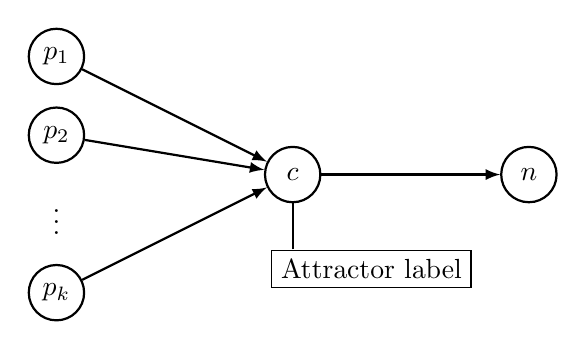
\begin{tikzpicture}[x=1cm, y=1cm]
		\vertex (p1) at (0,2) {$p_1$};
		\vertex (p2) at (0,1) {$p_2$};

		\vertex (p4) at (0,-1) {$p_k$};
		\vertex (c) at (3,0.5) {$c$};
		\vertex (n) at (6,0.5) {$n$};
		
		\draw [->,thick] 
		(p1) edge (c)
		(p2) edge (c)
		(p4) edge (c)
		(c) edge (n);
		\draw (0,0) node {$\vdots$};
		\draw (4,-0.7) node[rectangle,draw] {Attractor label};
		\draw [thick] (3,-0.45) -- (3,0.15);
		
		\end{tikzpicture}
	\par	
\end{figure}

\paragraph*{}
To fill the information in for every state, we have to obey the following steps. Remember that every state can be interpreted as a number. Using this, we begin by choosing the lowest yet not visited state and look at its evolution of the next time step. We can use this to store the next state's information to our current state and the current one is obviously a predecessor of the following one. We use the next state afterward as our current one and repeat the procedure. Thereby we always check if the following state has already been applied with a previous one. At this point, we would stop since it would mean one of two things.

\paragraph*{}
First, we could have reached a cycle and we get to know whether that is the case by looking at the next node attractor label. Because if it does not already belong to an attractor, the only way we could find an existing predecessor for the next time step would be that we have visited in this previous path. The other possibility would be that it already belongs to a basin of attraction.

\paragraph*{}
Either way, we start going backward and apply all the previous nodes with the attractor's label we either have hit on our path or, if we have found just a cycle, give them all a yet unused attractor label. If we have ended up at the state from which we started the path, we can start ones again from the now lowest not visited state. This way, we go through the whole phase space only about two times, one forward and one backward. The information we are interested in can either be collected during the run or afterward by iterating through the states with their full data. If we are interested in the in-degree of the states, the latter option would be the way to go.

\paragraph*{}
There are a few traps one could walk into if not being careful enough. One of them could be to naively implement the backward path so that it stops if there is no previous node anymore. If we initialized on a cycle, this would mean that we get stuck in an infinite loop. But checking if the previous node has an attractor label instead of just assigning it already fixes this.

\paragraph*{}
\chapter{Further Figures}
\section{Statistical Values for Critical Networks}
\begin{figure}[h!]
	\centering
	\begin{subfigure}{\textwidth}
		\includegraphics[width=\textwidth]{Plots/mvsk_N10_K2}
	\end{subfigure}
	\caption{Here we provide some statistical values with higher moments of the distributions of the critical networks (see Figure \ref{fig:new_scatter} on the right). This has been one of the first approaches in trying to understand the variations in the basin sizes. Since we could not find any useful information in this plots, we decided to separate them from our main work. So we decided to put them here for the interested reader.}
	\label{fig:statistical_values}
	\par
\end{figure}
\newpage
\section{Additional Plots to Figure \hyperref[fig:basin_sizes_main]{3.4}}
\begin{figure}[h!]
\begin{subfigure}{\textwidth}
\includegraphics[width=\textwidth]{Plots/basin_sizes_N10}
\end{subfigure}
\begin{subfigure}{\textwidth}
\includegraphics[width=\textwidth]{Plots/basin_sizes_N12}
\end{subfigure}
	\caption{Here we see plots like in Figure \ref{fig:basin_sizes_main}, only now for the sizes $N=10$ and $N=12$. The first were done over $10^7$ realizations and the second over $10^6$. The upper plots show the averaged normalized basins of attraction (orange) and the part that the garden-of-Eden states (green) take up from the whole phase space. Below them we have the probability distribution for attractors with length L to appear.}
	\label{fig:basin_sizes_main_additional_sizes}
\end{figure}

\begin{figure}[h!]
	\begin{subfigure}{\textwidth}
		\includegraphics[width=\textwidth]{Plots/basin_sizes_N10_frozen}
	\end{subfigure}
	\begin{subfigure}{\textwidth}
		\includegraphics[width=\textwidth]{Plots/basin_sizes_N10_chaotic}
	\end{subfigure}
	\caption{Here we see plots like in Figure \ref{fig:basin_sizes_main}, only now for the in-degrees $K\in \{1,1.3,1.7\}$ (frozen) and $K\in \{3,5,7\}$ (chaotic). All were done over $10^6$ realizations. The upper plots show the averaged normalized basins of attraction (orange) and the part that the garden-of-Eden states (green) take up from the whole phase space. Below them we have the probability distribution for attractors with length L to appear.}
	\label{fig:basin_sizes_main_additional_frozen_chaotic}
\end{figure}
\newpage
\paragraph*{}\paragraph*{}\paragraph*{}
\section{Additional Plots to Figure \hyperref[fig:basin_hists]{3.11}}\label{sec:basin_hists_additional}
\begin{figure}[h!]
	\begin{subfigure}{\textwidth}
		\includegraphics[width=\textwidth]{Plots/basin_hists_N7_2}
	\end{subfigure}
	\begin{subfigure}{\textwidth}
		\includegraphics[width=\textwidth]{Plots/basin_hists_N9_2}
	\end{subfigure}
	\caption{Those plots are the histograms from Figure \ref{fig:basin_hists} with system sizes $N=7$ and $N=9$.}
	\label{fig:basin_hists_additional_sizes}
\end{figure}

\begin{figure}[h!]
	\begin{subfigure}{\textwidth}
		\includegraphics[width=\textwidth]{Plots/basin_hists_N8_3}
	\end{subfigure}
	\begin{subfigure}{\textwidth}
		\includegraphics[width=\textwidth]{Plots/basin_hists_N8_4}
	\end{subfigure}
	\caption{Those plots are the histograms from Figure \ref{fig:basin_hists} with system size $N=8$ with the numbers of attractors $N_A=3$ and $N_A=4$.}
	\label{fig:basin_hists_additional_attractors}
\end{figure}

\newpage
\paragraph*{}\paragraph*{}
\section{Additional Plots to Figure \hyperref[fig:single_flip_stability]{3.13}}
\begin{figure}[h!]
	\begin{subfigure}{\textwidth}
		\includegraphics[width=\textwidth]{Plots/single_flip_stability_N10}
	\end{subfigure}
	\begin{subfigure}{\textwidth}
		\includegraphics[width=\textwidth]{Plots/single_flip_stability_N12}
	\end{subfigure}
	\caption{Those plots show the graphs of stability like in Figure \ref{fig:single_flip} with system sizes $N=10$ and $N=12$. We compare the stability of frozen $ N_f $ and active nodes $ N_a $. As we have seen before, the critical networks are where both groups of nodes are equally stable independent of the network size.}
	\label{fig:single_flip_additional}
\end{figure}



\bibliographystyle{abbrv}
\bibliography{bibfile}

\thispagestyle{empty}
\textbf{Erklärung} nach § 30 (12) Ordnung für den Bachelor- und dem Masterstudiengang\\
\vspace*{1cm}\\
Hiermit erkläre ich, dass ich die Arbeit selbstständig und ohne Benutzung anderer als der angegebenen Quellen und Hilfsmittel verfasst habe. Alle Stellen der Arbeit, die wörtlich oder sinngemäß aus Veröffentlichungen oder aus anderen fremden Texten entnommen wurden, sind von mir als solche kenntlich gemacht worden. Ferner erkläre ich, dass die Arbeit nicht - auch nicht auszugsweise - für eine andere Prüfung verwendet wurde. \\
\vspace*{2cm}\\
Frankfurt, den
\end{document}